\documentclass[a4j]{jarticle}
\usepackage[dvipdfmx]{graphicx}
\usepackage{here}
\usepackage{ascmac}
\usepackage{url}
\title{
\vspace{30mm}
株式会社マルナカ様\\
購入商品情報管理システム\\
内部設計書v2.0
\vspace{90mm}
}
\author{
株式会社Toron
}

\begin{document}
\maketitle
\newpage
\tableofcontents
\newpage


\section{システム概要}
本システムはマルナカを利用するユーザに対し、保有する食品や購入履歴などを簡単に管理できるようにするサービスを提供する。さらに、マルナカに対しては顧客の獲得を支援する「特売・特価情報通知」サービスを提供する。\par
本システムはAndroid端末を対象としたアプリケーション「マルナカ de お買い物♪」、アプリで提供する情報を管理する「管理者ページ」によって構築される。各要素の主な機能は以下に示す通りである。
\begin{itemize}
\item マルナカ de お買い物♪

\begin{itemize}
\item ユーザ情報の登録・認証
\item 保有食品の表示や更新・削除
\item 購入履歴の表示
\item 特売・特価情報の通知・表示
\item お気に入り店舗の登録
\end{itemize}

\item 管理者ページ

\begin{itemize}
\item 管理者ユーザ情報の認証
\item 店舗の登録と店舗情報の更新・削除
\item 特売情報の登録と更新・削除
\item 特価情報の登録
\item 特価商品が品切れになった際の品切れ商品登録
\end{itemize}

\end{itemize}
\section{動作環境}
本節では本システムの利用及び運用するために必要な環境を示す。
\subsection{マルナカ de お買い物♪}
マルナカ de お買い物♪の動作環境を表\ref{Dmarunaka}に示す。
\begin{table}[h]
  \begin{center}
    \caption{マルナカ de お買い物♪の動作環境}
    \begin{tabular}{|l|c|}\hline
      OS&Android 4.4以上\\ \hline
      必要機能&なし\\ \hline
      通信& 3G/4G(LTE)またはWi-Fiによるインターネット接続あり\\ \hline
      API&OpenGL 2.0以上 \\ \hline
    \end{tabular}
    \label{Dmarunaka}
  \end{center}
\end{table}

\newpage

\subsection{管理者ページ}
管理者ページの動作環境を表\ref{Dmaster}に示す。
\begin{table}[h]
  \begin{center}
    \caption{管理者ページの動作環境}
    \begin{tabular}{|l|c|}\hline
      OS&Windows10 home 64bit\\ \hline
      データベース&SQLite 3.26\\ \hline
      Webサーバ&Apache 2.4.33\\ \hline
    \end{tabular}
    \label{Dmaster}
  \end{center}
\end{table}

\subsection{サーバ}
サーバの動作環境を表\ref{Dsaba}に示す。
\begin{table}[h]
  \begin{center}
    \caption{サーバの動作環境}
    \begin{tabular}{|l|c|}\hline
      レンタル先&Amazon Web Service\\ \hline
      モデル&a1.xlarge\\ \hline
      メモリ&8GB\\ \hline
      ネットワーク帯域幅&最大10Gbps\\ \hline
      ストレージ&2TB\\ \hline
      virtual CPU&4vCPU\\ \hline
    \end{tabular}
    \label{Dsaba}
  \end{center}
\end{table}


\section{開発環境}
本節では本システム開発する際に必要な環境を示す。

\subsection{マルナカ de お買い物♪}
マルナカ de お買い物♪の開発環境を表\ref{Kmarunaka}に示す。
\begin{table}[h]
  \begin{center}
    \caption{マルナカ de お買い物♪の開発環境}
    \begin{tabular}{|l|c|}\hline
      IDE&Android Studio 4.0以上\\ \hline
      APIレベル&20以上\\ \hline
      開発言語&Java\\ \hline
      画面設計&XML\\ \hline

    \end{tabular}
    \label{Kmarunaka}
  \end{center}
\end{table}

\subsection{管理者ページ}
管理者ページの開発環境を表\ref{Kmaster}に示す。
\begin{table}[h]
  \begin{center}
    \caption{管理者ページの開発環境}
    \begin{tabular}{|l|c|}\hline
      開発言語&JAvascript + PHP 7\\ \hline
      データベース&SQLite 3.26\\ \hline
    \end{tabular}
    \label{Kmaster}
  \end{center}
\end{table}

\subsection{サーバ}
サーバの開発環境を表\ref{Ksaba}に示す。
\begin{table}[h]
  \begin{center}
    \caption{サーバの開発環境}
    \begin{tabular}{|l|c|}\hline
      開発言語&PHP 7\\ \hline
    \end{tabular}
    \label{Ksaba}
  \end{center}
\end{table}

\section{コーディング規約}

本節では本システムを開発する際のコーティング規約を示す。また、命名規則として英単語を使用する。
\subsection{Java}

本小節ではJavaを使用する際のコーディング規約を示す。1レベルインデントするごとに半角空白を4つ使用する。
\begin{itemize}
	\item クラス\\
		クラス名にはアッパーキャメルケース表記を使用する。
	\begin{itemize}
		\item 2つ以上の英単語を使用する
		\item 単語の頭文字は大文字を使用する
		\item 名称には英字のみを使用する
	\end{itemize}
		クラスの役割に応じて表 \ref{tab:o1} に示す単語を名称の最後に使用する。
		%
		\begin{table}[H]
			\caption{Javaのクラス名に使用する単語}
			\label{tab:o1}
			\begin{center}
			\begin{tabular}{|c|c|}
			\hline
			画面定義 & Activity\\\hline
			\end{tabular}
			\end{center}
			\end{table}
	\item メソッド\\
		メソッド名にはアッパーキャメルケース表記を使用する。
	\begin{itemize}
		\item 2つ以上の英単語を使用する
		\item 単語の頭文字は大文字を使用する
		\item 名称には英字のみを使用する
	\end{itemize}
		メソッドの実装に応じて表 \ref {tab:o2} に示す単語を名称の最初に使用する。
		%
				\begin{table}[H]
			\caption{Javaのメソッド名に使用する単語}
			\label{tab:o2}
			\begin{center}
			\begin{tabular}{|c|c|}
			\hline
			データの取得 & Get\\\hline
			データの設定 & Set\\\hline
			データの表示 & Display\\\hline
			データの並び替え & Sort\\\hline
			データの更新  & Updata\\\hline
			データの削除  & Delete\\\hline
			データの照合 & Check\\\hline
			\end{tabular}
			\end{center}
			\end{table}
	\item 変数・定数\\
		変数名または定数名にはアッパーキャメルケース表記を使用する。
	\begin{itemize}
		\item 2つ以上の英単語を使用する
		\item 単語の頭文字は大文字を使用する
		\item 名称には英字のみを使用する
	\end{itemize}


\end{itemize}
\subsection{Javascript}

本小節ではJavascriptのコーディング規約を示す。1レベルインデントするごとに半角空白を4つ使用する。

\begin{itemize}
	\item メソッド\\
		メソッド名にはアッパーキャメルケース表記を使用する。
	\begin{itemize}
		\item 2つ以上の英単語を使用する
		\item 単語の頭文字は大文字を使用する
		\item 名称には英字のみを使用する
	\end{itemize}
		メソッドの実装に応じて表 \ref {tab:o3} に示す単語を名称の最初に使用する。
				\begin{table}[H]
			\caption{Javascriptのメソッド名に使用する単語}
			\label{tab:o3}
			\begin{center}
			\begin{tabular}{|c|c|}
			\hline
			データの取得 & Get\\\hline
			データの設定 & Set\\\hline
			データの更新  & Updata\\\hline
			データの削除  & Delete\\\hline
			\end{tabular}
			\end{center}
			\end{table}
	\item 変数・定数\\
		変数名または定数名にはローワーキャメルケース表記を使用する。
	\begin{itemize}
		\item 2つ以上の英単語を使用する
		\item 名称の頭文字は小文字を使用し、後続する単語の頭文字は大文字を使用する
		\item 名称には英字のみを使用する
	\end{itemize}
\end{itemize}
\subsection{php}

本小節ではphpのコーディング規約を示す。1レベルインデントするごとに半角空白を4つ使用する。

\begin{itemize}
	\item メソッド\\
		メソッド名にはローワーキャメルケース表記を使用する。
	\begin{itemize}
		\item 2つ以上の英単語を使用する
		\item 名称の頭文字は小文字を使用し、後続する単語の頭文字は大文字を使用する
		\item 名称には英字のみを使用する
	\end{itemize}
		メソッドの実装に応じて表 \ref {tab:ophp} に示す単語を名称の最初に使用する。
				\begin{table}[H]
			\caption{phpのメソッド名に使用する単語}
			\label{tab:ophp}
			\begin{center}
			\begin{tabular}{|c|c|}
			\hline
			データの取得 & get\\\hline
			データの追加 & insert\\\hline
			データの更新  & dpdata\\\hline
			データの削除  & Delete\\\hline
			データの表示 &show\\\hline
			\end{tabular}
			\end{center}
			\end{table}
\end{itemize}
\subsection{データベース}
本小節ではデータベースのコーディング規約を示す。
	\begin{itemize}
	\item 共通\\
		スネークケース表記を使用する。
	\begin{itemize}
		\item 使用する文字は全て大文字とする
		\item 単語が連なる場合は後続する単語の前にアンダースコアを使用する
	\end{itemize}
	\item テーブル\\
		変数名または定数名にはローワーキャメルケース表記を使用する。
	\item カラム
		主キーの名称はテーブル名、アンダースコア、idで命名する。
\end{itemize}


\section{モジュール設計}
本節ではAndroid 版アプリケーション[マルナカdeお買い物]として、アプリケーションと管理者用webページ,サーバーのそれぞれのクラスが持つメソッド、入出力、またそれらの関係を示す。
本節で示す各モジュールはアプリケーション側の各画面である図\ref{tab:senni}とwebページ側の各画面である図\ref{tab:senni2}を構成する要素である.
\begin{figure}[H]
\begin{center}
\resizebox{16cm}{!}{\includegraphics{senni.PNG}}
\caption{アプリケーション遷移図}
\label{tab:senni}
\end{center}
\end{figure}
\begin{figure}[H]
\begin{center}
\resizebox{16cm}{!}{\includegraphics{senni2.PNG}}
\caption{webページ遷移図}
\label{tab:senni2}
\end{center}
\end{figure}

\subsection{モジュール設計(マルナカdeお買い物)}
本小節では、マルナカdeお買い物で実装するクラスとそのクラスが持つメソッドの解説とデータの遷移について記述する。また,以下にマルナカdeお買い物で実装する際のディレクトリ構造を図\ref{tab:directory}に示す.
\begin{figure}[H]
\begin{center}
\resizebox{16cm}{!}{\includegraphics{directory.PNG}}
\caption{マルナカdeお買い物のディレクトリ構造}
\label{tab:directory}
\end{center}
\end{figure}

\subsubsection{AuthenticationUser.Java}
\label{tab:Authentication}
ユーザ認証を行うクラスである。\\
%クラスの説明はもっといっぱい書く.ざっと7行くらい
メンバ変数として以下に示すオブジェクトを用いる。\\
\begin{itemize}
\item  private ArrayList\verb|<| User\verb|<|WaonNumber, SecureNumber,LoginID,Password,UserName\verb|>>| UserData
\item private DatabaseHelper mDatabaseHelper
\end{itemize}
本クラスのonCreateメソッドでは\ref{tab:DatabaseHelper}小節で示すDataBaseHelperクラスをインスタンス化し、メンバ変数mDataBaseHelperで管理する。\\
 本ActivityクラスのonResumeメソッドでの処理の流れを\ref{tabs:AuthenticationUser}小節の図\ref{tab:AuthenticationUser}に示す。\\
ユーザはログイン画面で登録されたログインIDとパスワードを入力し、認証が正しく行われると、\ref{tab:HoldingFood}小節に示すHoldingFoodActivityクラスで設計される保有食品画面へ遷移する。登録していないユーザは新規登録をタップすることで、\ref{tab:Registration}小節に示すRegistrationUserActivityクラスで設計される新規登録画面へ遷移する。
\begin{itemize}
\item メソッド名:CheckAuthenticationUser\\
  ユーザ認証を行うメソッドである。引数としてユーザ登録に必要な情報が格納されたArrayListオブジェクトとメンバ変数mDatabaseHelperを受け取る。戻り値としてboolean型変数Successを取得して返す。
  \begin{itemize}
  \item 引数1 : ArrayList\verb|<|User\verb|<|LoginID,Password\verb|>>| UserData
  \item 引数2 : DatabaseHelper mDatabaseHelper
  \item 戻り値:boolean Success
  \end{itemize}
\item メソッド名 : TransitionHomeActivity\\
  HomeActivityクラスへ遷移するメソッドである。
\begin{itemize}
  \item 引数 : なし
  \item 戻り値 : なし
\end{itemize}
\item メソッド名 : TransitionRegistrationUser\\
 ユーザ登録画面へ遷移するメソッドである.\\
\begin{itemize}
  \item 引数 : なし
  \item 戻り値 : なし
\end{itemize}
\end{itemize}


\subsubsection{RegistrationUser.Java}
\label{tab:Registration}
ユーザ登録を行うクラスである。\\
%クラスの説明はもっといっぱい書く.ざっと7行くらい
メンバ変数として以下に示すオブジェクトを用いる。
\begin{itemize}
\item private DatabaseHelper mDatabaseHelper
\end{itemize}
 本クラスのonCreateメソッドでは\ref{tab:DatabaseHelper}小節で示すDataBaseHelperクラスをインスタンス化し、メンバ変数mDataBaseHelperで管理する。\\
 本ActivityクラスのonResumeメソッドでの処理の流れを\ref{tabs:RegistrationUserForApplicationSequence}小節の図\ref{tab:RegistrationUserForApplicationSequence}に示す。\\
本Activityクラスはログイン画面で新規登録をタップしたときに表示される。ユーザはWAON番号とセキュリティコード、ログインID、ユーザ名、パスワードを入力し完了をタップすると、\ref{tab:HoldingFood}小節に示すHoldingFoodActivityクラスで設計される保有食品閲覧画面へ遷移する。
\begin{itemize}
\item メソッド名 : SetRegistrationUser\\
  登録情報をデータベースへ飛ばすメソッドである。\\
  引数としてユーザ登録に必要な情報が格納されたArrayListオブジェクトとメンバ変数mDatabaseHelperを受け取る。戻り値としてboolean型変数Successを取得して返す。
  \begin{itemize}
  \item 引数1 : ArrayList\verb|<|User\verb|<|WaonNumber,SecureNumber,LoginID,Password,UserName\verb|>>| UserData
  \item 戻り値 : boolean Success
  \end{itemize}
 \item メソッド名 : TransitionAuthenticationUser\\
  ユーザ認証画面へ遷移するメソッドである.\\
 \begin{itemize}
   \item 引数 : なし
   \item 戻り値 : なし
 \end{itemize}
\end{itemize}


\subsubsection{HomeActivity.Java}
\label{tab:Home}
ユーザがログインしているかの確認とローカルデータベース作成を行うクラスである。\\
 メンバ変数として以下に示すオブジェクトを用いる。
\begin{itemize}
\item private String UserID
\item private DatabaseHelper mDatabaseHelper
\end{itemize}
 本ActivityクラスのonCreateメソッドでは\ref{tab:DatabaseHelper}小節で示すDataBaseHelperクラスをインスタンス化し、メンバ変数mDataBaseHelperで管理する。\\
%%%%%ラベリングが必要
 本ActivityクラスのonResumeメソッドでの処理の流れを\ref{tabs:HomeActivityAndCreateLocalDatabaseSequence}小節の図\ref{tab:HomeActivityAndCreateLocalDatabaseSequence}に示す。\\
 本Activityクラスはユーザがアプリを開いた時点で表示される。ユーザが登録済みであれば\ref{tab:HoldingFood}小節に示すHoldingFoodActivityクラスで設計される保有食品閲覧画面へ遷移する。登録されていなユーザであれば、\ref{tab:Authentication}小節に示すAuthenticationActivityクラスで設計されるログイン画面へ遷移する。
\begin{itemize}
\item メソッド名:GetUserData\\
   ユーザーが既にログインしているかを判定するため、ローカルデータベースからユーザIDを取得するメソッドである。\\
   引数としてメンバ変数mDatabaseHelperを受け取り、戻り値としてString型変数UserIDを取得して返す。
  \begin{itemize}
  \item 引数:DatabaseHelper mDatabaseHelper
  \item 戻り値:String UserID
  \end{itemize}

\item メソッド名 : SetLocalDatabase\\
   UserIDが返ってきた場合、つまりローカルデータベースにUserテーブルが生成されている場合に呼び出され、ローカルデータベースを生成するメソッドである。\\
   引数としてメンバ変数mDatabaseHelperとString型変数UserIDを受け取り、戻り値としてboolean型変数Successを取得して返す。
  \begin{itemize}
  \item 引数 1:DatabaseHelper mDatabaseHelper
  \item 引数 2:String UserID
  \item 戻り値:boolean Success
  \end{itemize}

\item メソッド名 : TransitionHoldingFoodActivity\\
   初期表示画面である保有食品表示画面に遷移するメソッドである。
  \begin{itemize}
  \item 引数 : なし
  \item 戻り値 : なし
  \end{itemize}
\end{itemize}


\subsubsection{HoldingFoodActivity.Java}
\label{tab:HoldingFood}
ユーザーの保有食品を表示するクラスである。\\
 メンバ変数として以下に示すオブジェクトを用いる。
\begin{itemize}
\item private ArrayList\textless  HoldingFood\textless ProductName, Num, CreateDate\textgreater \textgreater  HoldingFoodData
\item private DatabaseHelper mDatabaseHelper
\end{itemize}
 本ActivityクラスのonCreateメソッドでは\ref{tab:DatabaseHelper}小節で示すDataBaseHelperクラスをインスタンス化し、メンバ変数mDataBaseHelperで管理する。\\
%%%%%ラベリングが必要
 本ActivityクラスのonResumeメソッドでの処理の流れを\ref{tabs:HoldingFoodSequence}小節の図\ref{tab:HoldingFoodSequence}に示す。このメソッド内で取得した購入履歴情報のデータはメンバ変数PurchaseHistoryDataで管理する。\\
 本Activityクラスはユーザがアプリにログインした時点で表示される。本Activityクラスで設計される画面下に赤い帯状の機能選択バーがある。「購入」をタップすることで、\ref{tab:PurchaseHistory}小節に示すPurchaseHistoryActivityクラスで設計される購入履歴閲覧画面へ遷移する。「特売・特価」をタップすることで\ref{tab:SpecialSale}小節に示すSpecialSaleActivityクラスで設計される特売情報閲覧画面に遷移する。その画面には「特売」と「特価」を選択するバーがあり、「特価」をタップすることで\ref{tab:SpecialPrice}小節に示すSpecialPriceActivityクラスで設計される特価情報閲覧画面に遷移する。「その他」をタップすることで、\ref{tab:Other}小節に示すOtherActivityクラスで設計されるその他画面へ遷移する。
\begin{itemize}
\item メソッド名:GetHoldingFoodData\\
   ユーザーの保有食品情報を取得するため、ローカルデータベースから保有食品情報を取得するメソッドである。\\
   引数としてメンバ変数mDatabaseHelperを受け取り、戻り値としてHoldingFoodDataを取得して返す。
  \begin{itemize}
  \item 引数:DatabaseHelper mDatabaseHelper
  \item 戻り値:HoldindFoodData
  \end{itemize}

\item メソッド名:DisplayHoldingFood\\
   ArrayList\textless  HoldingFood\textless ProductName, Num, CreateDate\textgreater \textgreater  HoldingFoodDataの長さの数だけループしユーザの保有食品情報を画面に表示するメソッドである。\\
   引数として保有食品情報を格納したArrayListオブジェクトを受け取る。
  \begin{itemize}
  \item 引数:HoldingFoodData
  \item 戻り値 : なし
  \end{itemize}

\item メソッド名:UpdateHoldingFoodCount\\
   商品の個数が変更されたとき、ユーザの保有食品テーブルから対象の商品の情報を更新するするメソッドである。\\
   引数として保有食品情報を格納したHoldingFoodオブジェクトを受け取り、戻り値としてboolean型変数Successを取得して返す。
  \begin{itemize}
  \item 引数:HoldingFood\textless ProductName, Num, CreateDate\textgreater
  \item 戻り値:boolean Success
  \end{itemize}

\item メソッド名:DeleteHoldingFoodCount\\
   商品の個数が0個になったとき、ユーザの保有食品テーブルから対象の商品を削除するメソッドである。\\
   引数として保有食品情報を格納したHoldingFoodオブジェクトを受け取り、戻り値としてboolean型変数Successを取得して返す。
  \begin{itemize}
  \item 引数:HoldingFood\textless ProductName, Num, CreateDate\textgreater
  \item 戻り値:boolean Success
  \end{itemize}

\item メソッド名:SortSyllabaly\\
   保有している商品を商品名の50音順に並び替えるメソッドである。\\
   引数として保有食品情報を格納したArrayListオブジェクトを受け取る。
  \begin{itemize}
  \item 引数:HoldingFoodData
  \item 戻り値 : なし
  \end{itemize}

\item メソッド名:SortCount\\
   保有している商品を商品の個数順に並び替えるメソッドである。\\
   引数として保有食品情報を格納したArrayListオブジェクトを受け取る。
  \begin{itemize}
  \item 引数:HoldingFoodData
  \item 戻り値 : なし
  \end{itemize}

\item メソッド名:SortDays\\
   保有している商品を商品の日付順に並び替えるメソッドである。\\
   引数として保有食品情報を格納したArrayListオブジェクトを受け取る。
  \begin{itemize}
  \item 引数:HoldingFoodData
  \item 戻り値 : なし
  \end{itemize}
\end{itemize}


\subsubsection{PurchaseHistoryActivity.Java}
\label{tab:PurchaseHistory}
ユーザの購入履歴を表示するクラスである。\\
 メンバ変数として以下に示すオブジェクトを用いる。
\begin{itemize}
\item private ArrayList\textless  PurchaseHistory\textless ProductName, Num, Price, CreateDate\textgreater \textgreater  PurchaseHistoryData
\item private DatabaseHelper mDatabaseHelper
\end{itemize}
 本ActivityクラスのonCreateメソッドでは\ref{tab:DatabaseHelper}小節で示すDataBaseHelperクラスをインスタンス化し、メンバ変数mDataBaseHelperで管理する。\\
%%%%%ラベリングが必要
 本ActivityクラスのonResumeメソッドでの処理の流れを\ref{tabs:AuthenticationUser}小節の図\ref{tab:PurchaseHistorySequence}に示す。このメソッド内で取得した購入履歴情報のデータはメンバ変数PurchaseHistoryDataで管理する。\\
 本Activityクラスで設計される画面下に赤い帯状の機能選択バーがある。「ホーム」をタップすることで、\ref{tab:HoldingFood}小節に示すHoldingFoodActivityクラスで設計される保有食品閲覧画面へ遷移する。「特売・特価」をタップすることで\ref{tab:SpecialSale}小節に示すSpecialSaleActivityクラスで設計される特売情報閲覧画面に遷移する。その画面には「特売」と「特価」を選択するバーがあり、「特価」をタップすることで\ref{tab:SpecialPrice}小節に示すSpecialPriceActivityクラスで設計される特価情報閲覧画面に遷移する。「その他」をタップすることで、\ref{tab:Other}小節に示すOtherActivityクラスで設計されるその他画面へ遷移する。
\begin{itemize}
\item メソッド名:GetPurchaseHistoryData\\
   ユーザの購入履歴に関する情報を取得するためのメソッドである。\\
   引数としてString型変数UserIDを受け取り、戻り値として購入履歴情報を格納したArrayListオブジェクトを取得して返す。
  \begin{itemize}
  \item 引数:String UserID
  \item 戻り値:PurchaseHistoryData
  \end{itemize}

\item メソッド名:DisplayPurchaseHistory\\
   ArrayList\textless  PurchaseHistory\textless ProductName, Num, Price, CreateDate\textgreater \textgreater  PurchaseHistoryDataの長さの数だけループし商品の購入履歴を画面に表示するメソッドである。\\
   引数として購入履歴情報を格納したArrayListオブジェクトを受け取る。
  \begin{itemize}
  \item 引数:PurchaseHistoryData
  \item 戻り値 : なし
  \end{itemize}
\end{itemize}


\subsubsection{SpecialSaleActivity.Java}
\label{tab:SpecialSale}
商品の特売情報を表示するクラスである。\\
 メンバ変数として以下に示すオブジェクトを用いる。
\begin{itemize}
\item private ArrayList\textless  SpecialSale\textless ProductName, Price\textgreater \textgreater  SpecialSaleData
\item private DatabaseHelper mDatabaseHelper
\end{itemize}
 本クラスのonCreateメソッドでは\ref{tab:DatabaseHelper}小節で示すDataBaseHelperクラスをインスタンス化し、メンバ変数mDataBaseHelperで管理する。\\
%%%%%ラベリングが必要
 本ActivityクラスのonResumeメソッドでの処理の流れを\ref{tabs:SpecialSaleSequence}小節の図\ref{tab:SpecialSaleSequence}に示す。このメソッド内で取得した特売情報のデータはメンバ変数SpecialSaleDataで管理する。\\
 本Activityクラスで設計される画面には「特売」と「特価」を選択するバーがあり、「特価」をタップすることで\ref{tab:SpecialPrice}小節に示すSpecialPriceActivityクラスで設計される特価情報閲覧画面に遷移する。また、画面下に赤い帯状の機能選択バーがある。「ホーム」をタップすることで、\ref{tab:HoldingFood}小節に示すHoldingFoodActivityクラスで設計される保有食品閲覧画面へ遷移する。「購入」をタップすることで、\ref{tab:PurchaseHistory}小節に示すPurchaseHistoryActivityクラスで設計される購入履歴閲覧画面へ遷移する。「その他」をタップすることで、\ref{tab:Other}小節に示すOtherActivityクラスで設計されるその他画面へ遷移する。
\begin{itemize}
\item メソッド名:GetSpecialSaleData\\
   商品の特売情報を取得するためのメソッドである。\\
   引数としてメンバ変数mDatabaseHelperを受け取り、戻り値として特売情報を格納したArrayListオブジェクトを取得して返す。
  \begin{itemize}
  \item 引数:DatabaseHelper mDatabaseHelper
  \item 戻り値:SpecialSaleData
  \end{itemize}

\item メソッド名:DisplaySpecialSale\\
   ArrayList\textless  SpecialSale\textless ProductName, Price\textgreater \textgreater  SpecialSaleDataの長さの数だけループし商品の特売情報を画面に表示するメソッドである。\\
   引数として特売情報を格納したArrayListオブジェクトを受け取る。
  \begin{itemize}
  \item 引数:SpecialSaleData
  \item 戻り値 : なし
  \end{itemize}
\end{itemize}


\subsubsection{SpecialPriceActivity.Java}
\label{tab:SpecialPrice}
商品の特価情報を表示するクラスである。\\
 メンバ変数として以下に示すオブジェクトを用いる。
\begin{itemize}
\item private ArrayList\textless  SpecialPrice\textless ProductName, DiscntVal, RateFlg, SoldOutFlg\textgreater \textgreater  SpecialPriceData
\item private DatabaseHelper mDatabaseHelper
\end{itemize}
 本ActivityクラスのonCreateメソッドでは\ref{tab:DatabaseHelper}小節で示すDataBaseHelperクラスをインスタンス化し、メンバ変数mDataBaseHelperで管理する。\\
%%%%%ラベリングが必要
 本ActivityクラスのonResumeメソッドでの処理の流れを\ref{tabs:SpecialPriceSequence}小節の図\ref{tab:SpecialPriceSequence}に示す。このメソッド内で取得した特価情報のデータはメンバ変数SpecialPriceDataで管理する。\\
 本Activityクラスで設計される画面には「特売」と「特価」を選択するバーがあり、「特売」をタップすることで\ref{tab:SpecialSale}小節に示すSpecialSaleActivityクラスで設計される特売情報閲覧画面に遷移する。また、画面下に赤い帯状の機能選択バーがある。「ホーム」をタップすることで、\ref{tab:HoldingFood}小節に示すHoldingFoodActivityクラスで設計される保有食品閲覧画面へ遷移する。「購入」をタップすることで、\ref{tab:PurchaseHistory}小節に示すPurchaseHistoryActivityクラスで設計される購入履歴閲覧画面へ遷移する。「その他」をタップすることで、\ref{tab:Other}小節に示すOtherActivityクラスで設計されるその他画面へ遷移する。
\begin{itemize}
\item メソッド名:GetSpecialPriceData\\
   商品の特価情報を取得するためのメソッドである。\\
   引数としてメンバ変数mDatabaseHelperを受け取り、戻り値として特価情報を格納したArrayListオブジェクトを取得して返す。
  \begin{itemize}
  \item 引数:DatabaseHelper mDatabaseHelper
  \item 戻り値:SpeciaPricelData
  \end{itemize}

\item メソッド名 : DisplaySpecialPrice\\
   ArrayList\textless  SpecialPrice\textless ProductName, DiscntVal, RateFlg, SoldOutFlg\textgreater \textgreater  SpecialPriceDataの長さの数だけループし商品の特価情報を画面に表示するメソッドである。\\
   引数として特価情報を格納したArrayListオブジェクトを受け取る。
  \begin{itemize}
  \item 引数:SpeciaPricelData
  \item 戻り値 : なし
  \end{itemize}
\end{itemize}


\subsubsection{OtherActivity.Java}%クラスの説明を追加
\label{tab:Other}
その他画面を表示するクラスである。\\
%%%%%ラベリングが必要
 本ActivityクラスのonResumeメソッドでの処理の流れを\ref{tabs:OtherSequence}小節の図\ref{tab:OtherSequence}に示す。\\
 本Activtyクラスで設計される画面には「店舗登録」と「パスワード変更」、「ログアウト」を選択するバーがある。「店舗登録」をタップすると\ref{tab:FavoriteShop}小節に示すFavoriteActivityクラスで設計される店舗登録画面に遷移する。「パスワード変更」をタップすると\ref{tab:ChangePassword}小節に示すChangePasswordActivityクラスで設計されるパスワード変更画面に遷移する。「ログアウト」をタップすると\ref{tab:Logout}小節に示すLogoutActivityクラスで設計されるログアウト画面に遷移する。
\begin{itemize}
\item メソッド名 : TransitionFavoriteShopActivity\\
  その他の画面から店舗登録画面に遷移するメソッドである。
  \begin{itemize}
  \item 引数 : なし
  \item 戻り値 : なし
  \end{itemize}

\item メソッド名 : TransitionChangePassowordActivity\\
  その他の画面からパスワード変更画面に遷移するメソッドである。
  \begin{itemize}
  \item 引数 : なし
  \item 戻り値 : なし
  \end{itemize}

\item メソッド名 : TransitionLogoutActivity\\
  その他の画面からログアウト画面に遷移するメソッドである。
  \begin{itemize}
  \item 引数 : なし
  \item 戻り値 : なし
  \end{itemize}
\end{itemize}


\subsubsection{FavoriteShopActivity.Java}
\label{tab:FavoriteShop}
店舗登録を行うクラスである。%クラスの説明を追加
メンバ変数を以下に示す。
\begin{itemize}
\item private DatabaseHelper mDatabaseHelper
\item private ArrayList\verb|<|FavoriteShop\verb|<|StoreID,Name,UserID\verb|>>| FavoriteShopData
\end{itemize}
本クラスのonCreateメソッドでは\ref{tab:DatabaseHelper}小節で示すDataBaseHelperクラスをインスタンス化し、メンバ変数mDataBaseHelperで管理する。\\
 本ActivityクラスのonResumeメソッドでの処理の流れを\ref{tabs:FavoriteShopSequence}小節の図\ref{tab:FavoriteShopSequence}に示す。このメソッド内で取得した店舗登録のデータはメンバ変数FavoriteShopDataで管理する。

\begin{itemize}
\item  メソッド名 : GetFavoriteShopData\\
  ユーザが登録している店舗の情報を取得するメソッドである。引数としてmDatabaseHelperを受け取り、戻り値としてArrayList型変数FavoriteShopDataを取得して返す。
  \begin{itemize}
  \item 引数 : DatabaseHelper mDatabaseHelper
  \item 戻り値 : FavoriteShopData
  \end{itemize}

\item メソッド名 : DisplayFavoriteShop\\
  ArrayList\verb|<| FavoriteShop\verb|<|StoreID,Name,UserID\verb|>>| FavoriteShopDataの長さの数だけループし、マルナカ全店舗の一覧を表示するメソッドである。引数としてArrayList型変数FavoriteShopDataの長さを取得し、戻り値としてboolean型変数Successを取得して返す。
  \begin{itemize}
  \item 引数 : FavoriteShopData
  \item 戻り値 : boolean Success
  \end{itemize}

\begin{itemize}
\item メソッド名 : UpdateFavoriteShopCount\\
  ユーザが登録した店舗を変更する動作を行うメソッドである。引数としてメンバ変数mDatabaseHelperとArrayList型変数FavoriteShopDataを受け取り、戻り値としてboolean型変数Successを取得して返す。
  \item 引数1 : FavoriteShopData
  \item 戻り値 : boolean Success
  \end{itemize}
\end{itemize}


\subsubsection{ChangePasswordActivity.Java}
\label{tab:ChangePassword}
パスワード変更、登録するクラスである。
メンバ変数を以下に示す。
\begin{itemize}
\item private DatabaseHelper mDatabaseHelper
\item private String LoginID
\item private String WaonNumber
\item private String SecureCode
\item private String Password
\end{itemize}
 本クラスのonCreateメソッドでは\ref{tab:DatabaseHelper}小節で示すDataBaseHelperクラスをインスタンス化し、メンバ変数mDataBaseHelperで管理する。\\
 本ActivityクラスのonResumeメソッドでの処理の流れを\ref{tabs:ChangePasswordSequence}小節の図\ref{tab:ChangePasswordSequence}に示す。
\begin{itemize}
\item メソッド名 : CheckCorrectUserData\\
  ユーザのログインID、WAON番号、セキュリティコードが正しいかローカルデータベースから判定するメソッドである。引数としてString型変数LoginID、String型変数WaonNumber、String型変数SecureCodeを受け取り、戻り値としてboolean型変数Correctを取得して返す。
  \begin{itemize}
  \item 引数1 : String LoginID
  \item 引数2 : String WaonNumber
  \item 引数3 : String SecureCode
  \item 戻り値:boolean Correct
  \end{itemize}

\item メソッド名 : ChangePassword\\
  ユーザが変更したパスワードをローカルデータベースに飛ばすメソッドである。引数としてString型変数Passwordを受け取り、戻り値としてboolean型変数successを取得して返す。
  \begin{itemize}
  \item 引数 : String Password
  \item 戻り値 : boolean success
  \end{itemize}

\item メソッド名 : TransitionOther\\
  パスワード変更が完了したときパスワード変更完了画面から、その他画面へ遷移するメソッドである。
  \begin{itemize}
  \item 引数 : なし
  \item 戻り値 : なし
  \end{itemize}
\end{itemize}

\subsubsection{LogoutActivity.Java}
\label{tab:Logout}
ログアウトをするクラスである。
メンバ変数を以下に示す。
\begin{itemize}
\item DatabaseHelper mDatabaseHelper
\end{itemize}
 本クラスのonCreateメソッドでは\ref{tab:DatabaseHelper}小節で示すDataBaseHelperクラスをインスタンス化し、メンバ変数mDataBaseHelperで管理する。\\
 本ActivityクラスのonResumeメソッドでの処理の流れを\ref{tabs:LogoutSequence}小節の図\ref{tab:LogoutSequence}に示す。
\begin{itemize}
\item メソッド名 : LogoutUser\\
  ログアウトするユーザのローカルデータベースのデータを削除するメソッドである。引数としてメンバ変数mDatabaseHelperを受け取る。
  \begin{itemize}
  \item 引数 : DatabaseHelper mDatabaseHelper
  \item 戻り値 : なし
  \end{itemize}

\item メソッド名 : TraisitionRegistrationUser\\
  ログアウト完了画面からユーザ登録画面へ遷移するメソッドである。
  \begin{itemize}
  \item 引数 : なし
  \item 戻り値 : なし
  \end{itemize}
\end{itemize}


\subsubsection{DatabaseHelper.java}
\label{tab:DatabaseHelper}

ローカルデータベースの生成とサーバーへの接続を行うクラスである。

\begin{itemize}

\item メソッド名 : MakeJSON

  引数として受け取ったJSONデータArrayList型変数ArrayList\textless Object\textgreater ArrayListDataを受け取り、JSONDataとして生成するメソッドである。戻り値はない。
  \begin{itemize}
  \item 引数 : ArrayList\textless Object\textgreater ArrayListData
		\item 戻り値 : なし
	\end{itemize}

    \item メソッド名 : CheckAuthenticationUser

	引数のJSONDataの中にはUserIDとPasswordが格納されており、このJSONDataをサーバに送信して認証を行うメソッドである。戻り値としてUserDataを格納したJSONDataが返される。

     \begin{itemize}
		\item 引数 : JSON JSONData
		\item 戻り値 : JSON JSONData
	\end{itemize}

     \item メソッド名 : CheckAuthenticationSuccess

	ユーザ認証に成功しているか、すなわちログインできているかをチェックするメソッドである。引数としてCheckAuthenticationUserで戻り値として受け取ったJSONDataを受け取り、中にUserDataが格納されているかどうかをチェックする。戻り値としてboolean型変数Successを返す。
      \begin{itemize}
		 \item 引数 : JSON JSONData
		 \item 戻り値 : boolean Success
	 \end{itemize}

     \item メソッド名 : SetUserData

	ユーザ情報をローカルデータベースに格納するメソッドである。引数としてJSONDataを受け取り、戻り値はない。
     \begin{itemize}
		\item 引数 : JSON JSONData
		\item 戻り値 : なし
	\end{itemize}

	\item メソッド名 : SetUserID

	ユーザIDをローカルデータベースに格納するメソッドである。戻り値としてString型変数UserIDを返す。
	\begin{itemize}
		\item 引数 : なし
		\item 戻り値 : String UserID
	\end{itemize}

	\item メソッド名 : CheckLocalDatabaseTable

	アプリ内でUserData以外のローカルデータベースが生成されているかどうかをチェックするメソッドである。引数はなく、戻り値としてboolean型変数Successを返す。
	\begin{itemize}
		\item 引数 : なし
		\item 戻り値 : boolean Success
	\end{itemize}

	\item メソッド名 : CleateLocalDatabaseTable

	ローカルデータベースを生成するメソッドである。戻り値はない。
	\begin{itemize}
		\item 戻り値 : なし
	\end{itemize}

	\item メソッド名 : GetLocalDataBase

	ローカルデータベースに必要なデータをサーバーに要求するメソッドである。引数としてString型変数UserIDを受け取り、戻り値としてJSONDataを取得して返す。戻り値のJSONDataには、ローカルデータベースの生成に必要なHoldingFoodテーブルとCategolyテーブルとFavoriteShopテーブルが格納されている。
	\begin{itemize}
		\item 引数 : String UserID
		\item 戻り値 : JSON JSONData
	\end{itemize}

	\item メソッド名 : SetHoldingFoodTable

	保有食品テーブルをローカルデータベースに格納するメソッドである。引数としてGetLocalDataBaseで戻り値として受け取ったJSONDataを受け取り、戻り値はない。
	\begin{itemize}
		\item 引数 : JSON JSONData
		\item 戻り値 : なし
	\end{itemize}

	\item メソッド名 : SetCategoryTable

	カテゴリテーブルをローカルデータベースに格納するメソッドである。引数としてGetLocalDataBaseで戻り値として受け取ったJSONDataを受け取り、戻り値はない。
	\begin{itemize}
		\item 引数 : JSON JSONData
		\item 戻り値 : なし
	\end{itemize}

	\item メソッド名 : SetShopTable

	店舗テーブルをローカルデータベースに格納するメソッドである。引数としてGetLocalDataBaseで戻り値として受け取ったJSONDataを受け取り、戻り値はない。
	\begin{itemize}
		\item 引数 : JSON JSONData
		\item 戻り値 : なし
	\end{itemize}

    \item メソッド名 : IsEnvironmentTableTime

	前回の更新から60秒経過しているか判定するメソッドである。引数はなく、戻り値としてboolean型変数Successを返す。
	\begin{itemize}
		\item 引数 : なし
		\item 戻り値 : boolean Success
	\end{itemize}

    \item メソッド名 : GetPurchaseHistoryData

	購入履歴テーブルに必要なデータをサーバに要求するメソッドである。引数としてString型変数UserIDを受け取り、戻り値としてJSONDataを取得して返す。戻り値のJSONDataには、ローカルデータベースの生成に必要なHoldingFoodテーブルとCategolyテーブルとFavoriteShopテーブルが格納されている。
    \begin{itemize}
		\item 引数 : String UserID
		\item 戻り値 : JSON JSONData
	\end{itemize}

    \item メソッド名 : CheckAdditionalPurchaseHistoryTable

	購入履歴テーブルの更新があるかを確認するメソッドである。引数としてGetPurchaseHistoryDataで戻り値として受け取ったJSONDataを受け取り、戻り値としてboolean型変数Successを返す。
	\begin{itemize}
		\item 引数 : JSON JSONData
		\item 戻り値 : boolean Success
	\end{itemize}

     \item メソッド名 : SetAdditionalPurchaseHistoryTable

	追加されたレコードを購入履歴テーブルに挿入するメソッドである。引数としてGetLocalDataBaseで戻り値として受け取ったJSONDataを受け取り、戻り値はない。
     \begin{itemize}
		\item 引数 : JSON JSONData
		\item 戻り値 : なし
	\end{itemize}

     \item メソッド名 : TotalCalculationMoney

	合計金額の再計算を行うメソッドである。引数と戻り値はない。
	\begin{itemize}
		\item 引数 : なし
		\item 戻り値 : なし
	\end{itemize}

	\item メソッド名 : SetPurchaseHistoryTable

	ローカルデータベースに格納されている購入履歴テーブルからArrayListを生成するメソッドである。引数と戻り値はない。
	\begin{itemize}
		\item 引数 : なし
		\item 戻り値 : なし
	\end{itemize}

	\item メソッド名 : GetHoldingFoodTable

	保有食品テーブルをローカルデータベースに格納するメソッドである。引数はなく、戻り値としてHoldingFoodDataを返す。
	\begin{itemize}
		\item 引数 : なし
		\item 戻り値 : HoldingFoodData
	\end{itemize}

	\item メソッド名 : SetUpdateHoldingFoodData

	保有食品内のある食品の個数が変動した時に保有食品テーブルの個数を更新するメソッドである。引数としてJSONDataを受け取り、戻り値としてboolean型変数Successを取得して返す。引数のJSONDataには、保有食品テーブルの更新に必要なHoldingFoodDataが格納されている。
	\begin{itemize}
		\item 引数 : JSON JSONData
		\item 戻り値 : boolean Success
	\end{itemize}

	\item メソッド名 : SetDeleteHoldingFoodData

	保有食品内のある食品の個数が0個になった時に食品を削除するメソッドである。引数としてJSONDataを受け取り、戻り値としてboolean型変数Successを取得して返す。引数のJSONDataには、削除に必要なHoldingFoodDataが格納されている。
	\begin{itemize}
		\item 引数 : JSON JSONData
		\item 戻り値 : boolean Success
	\end{itemize}

	\item メソッド名 : CheckFirstTimeOrUpdateTiming

	特売情報の表示に関して1回目もしくは更新される時間かどうか判定するメソッドである。引数はなく、戻り値としてboolean型変数Successを返す。
	\begin{itemize}
		\item 引数 : なし
		\item 戻り値 : boolean Success
	\end{itemize}

	\item メソッド名 : GetSpecialSaleData

	特売テーブルに必要なデータをサーバに要求するメソッドである。引数はなく、戻り値としてJSONDataを取得して返す。戻り値のJSONDataには、ローカルデータベースの生成に必要なProductテーブルが格納されている。
	\begin{itemize}
		\item 引数 : なし
		\item 戻り値 : JSON JSONData
	\end{itemize}

	\item メソッド名 : UpdateSpecialSaleTable

	特売テーブルの情報をすべて更新するメソッドである。引数としてGetSpecialSaleDataで戻り値として受け取ったJSONDataを受け取り、戻り値はない。
     \begin{itemize}
		\item 引数 : JSON JSONData
		\item 戻り値 : なし
	\end{itemize}

	\item メソッド名 : SetSpecialSaleTable

	特売テーブルをローカルデータベースに格納するメソッドである。引数と戻り値はない。
	\begin{itemize}
		\item 引数 : なし
		\item 戻り値 : なし
	\end{itemize}

	\item メソッド名 : GetSpecialPriceData

	特価テーブルに必要なデータをサーバに要求するメソッドである。引数はなく、戻り値としてJSONDataを取得して返す。戻り値のJSONDataには、ローカルデータベースの生成に必要なSpecialPriceテーブルとProductテーブルが格納されている。
	\begin{itemize}
		\item 引数 : なし
		\item 戻り値 : JSON JSONData
	\end{itemize}

	\item メソッド名 : UpdateSpecialPriceTable

	特価テーブルの情報をすべて更新するメソッドである。引数としてGetSpecialPriceDataで戻り値として受け取ったJSONDataを受け取り、戻り値はない。
     \begin{itemize}
		\item 引数 : JSON JSONData
		\item 戻り値 : なし
	\end{itemize}

	\item メソッド名 : SetSpecialPriceTable

	特価テーブルをローカルデータベースに格納するメソッドである。引数と戻り値はない。
	\begin{itemize}
		\item 引数 : なし
		\item 戻り値 : なし
	\end{itemize}

	\item メソッド名 : GetFavoriteShopData

	お気に入り店舗テーブルに必要なデータをサーバに要求するメソッドである。引数はなく、戻り値としてJSONDataを取得して返す。戻り値のJSONDataには、ローカルデータベースの生成に必要なUserテーブルが格納されている。
	\begin{itemize}
		\item 引数 : なし
		\item 戻り値 : JSON JSONData
	\end{itemize}

	\item メソッド名 : CheckAdditionalFavoriteShopTable

	お気に入り店舗テーブルの更新があるかを確認するメソッドである。引数としてGetFavoriteShopDataで戻り値として受け取ったJSONDataを受け取り、戻り値はない。
	\begin{itemize}
		\item 引数 : JSON JSONData
		\item 戻り値 : なし
	\end{itemize}

     \item メソッド名 : SetAdditionalFavoriteShopTable

	追加されたレコードをお気に入り店舗テーブルに挿入するメソッドである。引数としてGetFavoriteShopDataで戻り値として受け取ったJSONDataを受け取り、戻り値はない。
     \begin{itemize}
		\item 引数 : JSON JSONData
		\item 戻り値 : なし
	\end{itemize}

	\item メソッド名 : SetFavoriteShopTable

	お気に入り店舗テーブルをローカルデータベースに格納するメソッドである。引数と戻り値はない。
	\begin{itemize}
		\item 引数 : なし
		\item 戻り値 : なし
	\end{itemize}

	\item メソッド名 : SetUpdateFavoriteShopData

	お気に入り店舗を登録または変更した時にお気に入り店舗テーブルを更新するメソッドである。引数としてJSONDataを受け取り、戻り値としてboolean型変数Successを取得して返す。引数のJSONDataには、更新に必要なFavoriteShopDataが格納されている。
	\begin{itemize}
		\item 引数 : JSON JSONData
		\item 戻り値 : boolean Success
	\end{itemize}

	\item メソッド名 : SetNewPassword

	新しいパスワードをサーバへ送信するメソッドである。引数としてString型変数Passwordを受け取り、戻り値としてboolean型変数Successを取得して返す。
        \begin{itemize}
	\item 引数 : String Password
	\item 戻り値 : boolean Success
	\end{itemize}

      \item メソッド名 : DestroyLocalDatabase

	ログアウトの際にローカルデータベースを消去するメソッドである。引数と戻り値はない。
	\begin{itemize}
	\item 引数 : なし
	\item 戻り値 : なし
	\end{itemize}

	\item メソッド名 : TransitionFinishLogout

	ログアウトが完了したことを示すメソッドである。引数と戻り値はない。
	\begin{itemize}
		\item 引数 : なし
		\item 戻り値 : なし
	\end{itemize}


\end{itemize}
\subsection{モジュール設計(Webページ及びサーバー)}

本節ではWebページ及びサーバーのモジュール設計を示す。また、本システムで用いるサーバのディレクトリ構造を図\ref{tab:oonishimoj}に示す。

\begin{figure}[H]
\begin{center}
\resizebox{16cm}{!}{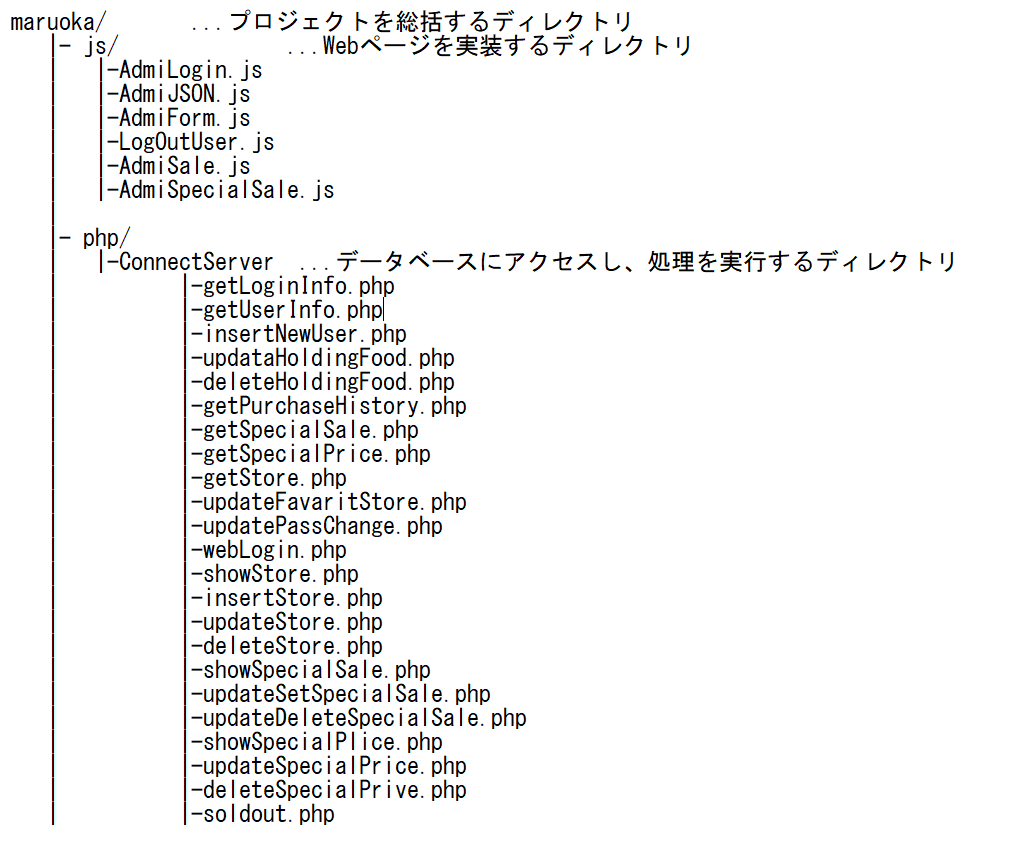
\includegraphics{webmoj.PNG}}
\caption{モジュール構成図}
\label{tab:oonishimoj}
\end{center}
\end{figure}
\subsection{管理者ページmaruokaディレクトリ}
webに関するすべての機能に関連するファイルが設置されているディレクトリである。\\
本小節では内包されている各ファイルについて示す。
\subsubsection{AdmiLogin.js}
ログイン画面を提供し、ユーザ情報に伴いページの遷移を行うクラスである。
\begin{itemize}

\item メソッド名:AuthentivationUsed\\

Webページでログインする際に、入力されたログイン情報がデータベースに登録されているか問い合わせを行うメソッドである。\\
引数として、入力されたユーザIDとパスワードを受け取る。\\
また戻り値はIdentifivationNumberである。これは、データベース上にログイン情報が存在したか判定を行った結果を返すものである。\\

	\begin{itemize}
		\item 引数1:userID
		\item 引数2:password
		\item 戻り値:IdentifivationNumber
	\end{itemize}
	\subsubsection{AdmiJSON.js}
入力された内容をデータベースに転送を行うクラスである。
\item メソッド名:SetJSON\\

JSONファイルを作成するメソッドである。\\引数は、ユーザIDとパスワードである。\\生成したJSONファイルを戻り値とする。
	\begin{itemize}
		\item 引数1:userID
		\item 引数2:password
		\item 戻り値:JSONData
	\end{itemize}
\item メソッド名:GetAutheticationUser\\

サーバーにJSONファイルを送信するためのメソッドである。\\
引数はAdmiJSON.jsで生成されたJSONDataである。
	\begin{itemize}
		\item 引数1:JSONData
	\end{itemize}

%サーバー側
\item メソッド名:CheckAutheticationUser\\

サーバ内で該当するユーザ情報が登録されているかJSONファイルをもとに検索するメソッドである。\\
引数はJSONDataである。\\
戻り値はIdentifivationNumberである。この変数の値は次のような意味を示す。
	\begin{itemize}
		\item 値が1:ユーザが店長である場合
		\item 値が2:ユーザが管理者である場合
		\item 値が0:入力されたユーザ情報と該当するユーザが存在しないなどのエラー
	\end{itemize}


\item メソッド名:ChangePage\\

引数の値に応じてページの遷移を行うメソッドである。\\
引数はIdentifivationNumberである。

	\begin{itemize}
		\item 引数1:IdentifivationNumber
	\end{itemize}
\subsubsection{AdmiForm.js}
ユーザに店舗の登録ページを提供し、登録された内容を表示を行うクラスである。

\item メソッド名:GetShopData\\

現在登録されている店舗情報をサーバから取得するためのメソッドである。このメソッドは、webページを開いた時点で呼ばれる。\\
引数はなく、戻り値はJSONDataとなる。
	\begin{itemize}
		\item 戻り値:JSONData
	\end{itemize}

\item メソッド名:CleateTable\\
JSONデータや入力情報をもとにWebページ上で表を作成するメソッドである。\\
引数として、JSONData内の店舗ID、店舗名、店長のユーザIDのデータもしくは、フォームに入力されたこれらのデータを受け取る。
	\begin{itemize}
		\item 引数1:shopID
		\item 引数2:shopName
		\item 引数3:userID
	\end{itemize}
\item メソッド名:RegistrationShop\\

追加の店舗情報をデータベースに登録するメソッドである。\\
引数は店舗IDと店舗名、店長のユーザIDである。\\
戻り値はboolean型のsuccessである。
	\begin{itemize}
		\item 引数1:shopID
		\item 引数2:shopName
		\item 引数3:userID
		\item 戻り値:success
	\end{itemize}
また戻り値の値の意味は次に示す。
	\begin{itemize}
		\item 値が0:データベースに正しく値が書き込めなかった場合
		\item 値が1:データベース更新成功
	\end{itemize}


\item メソッド名:UpdateShop\\

店舗情報を変更する際の処理を行うメソッドである。\\
引数は店舗IDと店舗名、店長のユーザIDである。\\
戻り値はboolean型のsuccessである。
	\begin{itemize}
		\item 引数1:shopID
		\item 引数2:shopName
		\item 引数3:userID
		\item 戻り値:success
	\end{itemize}
また戻り値の値の意味は次に示す。
	\begin{itemize}
		\item 値が0:データベースに正しく値が書き換えれなかった場合
		\item 値が1:データベース更新成功
	\end{itemize}

\item メソッド名:UpdateShop\\

サーバーにJSONファイルを送信するためのメソッドである。\\
引数はJSONDataである。
	\begin{itemize}
		\item 引数1:JSONData
	\end{itemize}

\item メソッド名:UpdateTable\\

データベース上で変更が完了したらWebページ上の店舗一覧に変更を加えるメソッドである。\\
引数として入力された店舗情報を受け取る。\\
戻り値はない。

	\begin{itemize}
		\item 引数1:shopID
		\item 引数2:shopName
		\item 引数3:userID
	\end{itemize}

\item メソッド名:DeleteShop\\

店舗情報を削除する際の処理を行うメソッドである。\\
引数は店舗IDと店舗名、店長のユーザIDである。\\
戻り値はboolean型のsuccessである。

	\begin{itemize}
		\item 引数1:shopID
		\item 引数2:shopName
		\item 引数3:userID
		\item 戻り値:success
	\end{itemize}
また戻り値の値の意味は次に示す。
	\begin{itemize}
		\item 値が0:データベース上から正しく削除できなかった場合
		\item 値が1:データベースから削除成功
	\end{itemize}

\item メソッド名:DeleteTable\\

表から削除が完了したデータを削除するメソッドである。\\
引数は店舗IDと店舗名、店長のユーザIDである。\\
戻り値はない。
	\begin{itemize}
		\item 引数1:shopID
		\item 引数2:shopName
		\item 引数3:userID
	\end{itemize}
\subsubsection{AdmiJSON.js}

登録された内容をデータベースに転送を行うための
クラスである。

\item メソッド名:SetJSON\\

店舗情報を変更する際に変更情報をサーバに送信するためにJSONファイルを作成するメソッドである。\\
引数は店舗IDと店舗名、店長のユーザIDである。\\
戻り値はJSONDataである。
	\begin{itemize}
		\item 引数1:shopID
		\item 引数2:shopName
		\item 引数3:userID
		\item 戻り値:JSONData
	\end{itemize}
\subsubsection{LogOutUser.js}

ログイン状態であるユーザのログアウト処理を行うためのクラスである。
%
\item メソッド名:LogOutUser\\

ログアウトボタンを押すと、ログイン前の状態に遷移する動作をさせるメソッドである。\\
引数と戻り値はない。
%
\subsubsection{AdmiLogin.js}

特売情報の登録・削除画面を提供するクラスである。
\item メソッド名:GetSaleData\\

登録済みの特売情報をJSONファイルで取得するメソッドである。\\
引数はない。\\
戻り値はJSONファイルである。
%中の表作成に必要なデータと、カテゴリーと商品名
	\begin{itemize}
		\item 戻り値:JSONData
	\end{itemize}


\item メソッド名:CleateTable\\

JSONデータや入力情報をもとにWebページ上で表を作成するメソッドである。\\
引数として、JSONData内の店舗ID、店舗名、店長のユーザIDもしくは、フォームに入力されたデータを受け取る。
	\begin{itemize}
		\item 引数1:shopID
		\item 引数2:shopName
		\item 引数3:userID
		\item 戻り値:success
	\end{itemize}
\item メソッド名:SetChoice\\

カテゴリーと商品名の選択肢を作成するメソッドである。\\
引数はJSONDataであり、JSONファイル中のカテゴリ名と商品名を必要とする。\\
戻り値はない。
	\begin{itemize}
		\item 引数1:JSONData
	\end{itemize}

\item メソッド名:SetRegistrationSale\\

特売にする商品のデータベースに登録を行うメソッド\\
引数は商品IDである。\\%かな?\\
戻り値はboolean型のsuccessである。

	\begin{itemize}
		\item 引数1:RegistrationID
		\item 戻り値:success
	\end{itemize}
また戻り値の値の意味は次に示す。
	\begin{itemize}
		\item 値が0:データベース上から正しく登録できなかった場合
		\item 値が1:データベースに登録成功
	\end{itemize}
\item メソッド名:SetDeleteSale\\

特売にする商品のデータベースから削除を行うメソッドである。\\
引数は商品IDである。\\
戻り値はboolean型のsuccessである。

	\begin{itemize}
		\item 引数1:RegistrationID
		\item 戻り値:success
	\end{itemize}
また戻り値の値の意味は次に示す。
	\begin{itemize}
		\item 値が0:データベース上から正しく削除できなかった場合
		\item 値が1:データベースに削除成功
	\end{itemize}
	\subsubsection{AdmiJSON.js}

入力された内容からJSONファイルを作成し、それをデータベースに転送を行うクラスである。\\

\item メソッド名:SetJSON\\

JSONファイルを作成するメソッドである。\\
引数は商品IDである。\\
戻り値はJSONDataである。
	\begin{itemize}
		\item 引数1:productID
		\item 戻り値:JSONData
	\end{itemize}
\subsubsection{AdmiLogin.js}

特価情報の登録・更新・削除画面を提供するクラスである。
%
\item メソッド名:GetSpecialSaleData\\

登録済みの特価情報をJSONファイルで取得するメソッドである。\\
引数はない。\\
戻り値はJSONファイルである。


	\begin{itemize}
		\item 引数1:JSONData
	\end{itemize}
	\item メソッド名:CleateTable\\

JSONデータや入力情報をもとにWebページ上で表を作成するメソッドである。\\
引数として、JSONData内の店舗ID、店舗名、店長のユーザIDもしくは、フォームに入力されたデータを受け取る。
	\begin{itemize}
		\item 引数1:shopID
		\item 引数2:shopName
		\item 引数3:userID
	\end{itemize}
\item メソッド名:SetChoice\\

カテゴリーと商品名の選択肢を作成するメソッドである。\\
引数はJSONDataであり、JSONファイル中のカテゴリ名と商品名を必要とする。\\
戻り値はない。
	\begin{itemize}
		\item 引数1:shopID
		\item 引数2:productID
	\end{itemize}

\item メソッド名:SetRegistrationSpecialSale\\

特価にする商品のデータベースに登録を行うメソッドである。\\
引数は店舗IDと商品IDと割引率と割引フラグである。\\
戻り値はboolean型のsuccessである。
	\begin{itemize}
		\item 引数1:shopID
		\item 引数2:productID
		\item 引数3:rate
		\item 引数4:rateFlag
	\end{itemize}
また戻り値の値の意味は次に示す。
	\begin{itemize}
		\item 値が0:データベース上から正しく登録できなかった場合
		\item 値が1:データベースに登録成功
	\end{itemize}
%
\item メソッド名:SetDeleteSpecialSale\\

特価にする商品のデータベースに削除を行うメソッドである。\\
引数は店舗IDと商品IDと割引率と割引フラグである。\\
戻り値はboolean型のsuccessである。
	\begin{itemize}
		\item 引数1:shopID
		\item 引数2:productID
		\item 引数3:rate
		\item 引数4:rateFlag
	\end{itemize}
また戻り値の値の意味は次に示す。
	\begin{itemize}
		\item 値が0:データベース上から正しく削除できなかった場合
		\item 値が1:データベースに削除成功
	\end{itemize}
%
\item メソッド名:SetUpdateSpecialeSale\\

売り切れた特価商品にイベントを起こすメソッドである。この際にデータベースのsoldoutの更新も行う。\\
引数は店舗IDと商品IDである。\\
戻り値はboolean型のsuccessである。
	\begin{itemize}
		\item 引数1:shopID
		\item 引数2:productID
	\end{itemize}
また戻り値の値の意味は次に示す。
	\begin{itemize}
		\item 値が0:データベース上から正しく更新できなかった場合
		\item 値が1:データベースに更新成功
	\end{itemize}

\subsubsection{AdmiJSON.js}

入力された内容からJSONファイルを作成し、それをデータベースに転送を行うためのクラスである。\\

\item メソッド名:SetJSON\\

JSONファイルを作成するメソッドである。\\
引数は店舗ID、商品ID、割引率と割引フラグである。\\
戻り値はJSONDataである。
	\begin{itemize}
		\item 引数1:shopID
		\item 引数2:productID
		\item 引数3:rate
		\item 引数4:rateFlag
	\end{itemize}
	\begin{itemize}
		\item 戻り値:JSONData
	\end{itemize}
\end{itemize}

%\subsection{モジュール設計(サーバー)}
%本小節では、サーバーで実装するクラスとメソッドの解説とデータの遷移について記述する。

\subsection{ConnectServerディレクトリ}
データベースにアクセスし処理を行うファイルが設置されているディレクトリである。
\begin{itemize}
\item getLoginInfo.php \\
  アプリでログイン時に認証に必要な情報をJSONファイルにまとめてアプリに返すためのファイルである。
  データベースにあるユーザテーブルにアクセスし、取得したユーザの値をJSONファイルにまとめる。
		\item getUserInfo.php \\
		アプリ内で持つ情報をJSONファイルにまとめてアプリに返すファイルである。
		データベースにある商品テーブル、保有食品テーブル、カテゴリーテーブルと店舗テーブルにアクセスし、取得した値をJSONファイルにまとめる。
		商品テーブルと保有食品テーブルを連結しユーザIDで検索を行い、その中の商品名、フリガナ、商品個数と作成日時を取得する。
		カテゴリーテーブルxでは、作成日時と更新日時以外の値を取得する。店舗テーブルでは、作成日時以外の値を取得する。
		\item insertNewUser.php \\
		ユーザが新規登録を行った際にユーザ情報を新たに追加するためのファイルである。
		ユーザの情報はJSONファイルで取得する。
		\item updateHoldingFood.php \\
		保有食品内のある食品の個数が変動した時にデータベースに個数の更新を行うファイルである。
		JSONファイルで取得した情報を基に保有食品テーブルの情報の更新を行う。
		\item deleteHoldingFood.php \\
		保有食品内のある食品の個数が0個になった時にデータベースから削除するファイルである。
		JSONファイルで取得した情報を基に保有食品テーブルのレコードの削除を行う。
		\item getPurchaseHistory.php \\
		購入履歴の情報をJSONファイルにまとめてアプリに返すファイルである。
		データベースの購入テーブルと商品テーブルにアクセスし、取得した値をJSONファイルにまとめる。
		購入テーブルと商品テーブルを連結しユーザIDで検索を行い、商品名、購入個数、作成日時を取得する。
		\item getSpecialSale.php \\
		特売情報をJSONファイルにまとめてアプリに返すファイルである。
		データベースの商品テーブルにアクセスし、取得した値をJSONファイルにまとめる。
		商品テーブルで特売の状態になっている商品を検索し、商品名と価格を取得する。
		\item getSpecialPrice.php \\
		特価情報をJSONファイルにまとめアプリに返すファイルである。
		データベースの特価テーブルと商品テーブルにアクセスし、取得した値をJSONファイルにまとめる。
		特価テーブルと商品テーブルを連結し、商品名、価格、割引値、割引率フラグを取得する。
		\item getStore.php \\
		店舗の情報をJSONファイルにまとめアプリに返すファイルである。
		データベースの店舗テーブルにアクセスし、取得した値をJSONファイルにまとめる。
		店舗テーブルの作成日時と更新日時以外の値を取得する。
		\item updateFavaritStore.php \\
		お気に入り店舗を登録または変更した際にデータベースにお気に入り店舗の情報の更新を行うファイルである。
		データベースのユーザテーブルにアクセスし、JSONファイルから取得した情報を基に情報を更新する。
		\item updatePassChange.php \\
		パスワードの変更を行った際にデータベースにパスワードの更新を行うファイルである。
		データベースのユーザテーブルにアクセスし、JSONファイルから取得した情報を基に情報を更新する。
		\item webLogin.php \\
		Webページで管理者(店長)がログインする時に認証を行うファイルである。
		\item showStore.php \\
		登録されている店舗情報をWeb画面に表示するための情報をJSONファイルにまとめるファイルである。
		データベースの店舗テーブルにアクセスし、取得した値をJSONファイルにまとめる。
		店舗テーブルの作成日時と更新日時以外の値を取得する。
		\item insertStore.php \\
		店舗情報を新たに追加するファイルである。
		JSONファイルで取得した情報を基に店舗テーブルに新たなレコードを追加する。
		\item updateStore.php \\
		店舗情報の更新を行うファイルである。
		JSONファイルで取得した情報を基に店舗テーブルを更新する。
		\item deleteStore.php \\
		店舗情報をデータベースから削除するファイルである。
		JSONファイルで取得した情報を基に店舗テーブルの指定されたレコードを削除する。
		\item showSpecialSale.php \\
		登録されている特売情報をWeb画面に表示するための情報をJSONファイルにまとめるファイルである。
		データベースの商品テーブルにアクセスし、取得した値をJSONファイルにまとめる。
		商品テーブルで特売の状態になっている商品を検索し、商品名と価格を取得する。
		\item updateSetSpecialSale.php \\
		指定された非特売商品を特売商品へ更新を行うファイルである。
		JSONファイルで取得した情報を基に商品テーブルの更新を行う。
		\item updateDeleteSpecialSale.php \\
		指定された特売商品を非特売商品へ更新を行うファイルである。
		JSONファイルで取得した情報を基に商品テーブルの更新を行う。
		\item showSpecialPlice.php \\
		登録されている特価情報をWeb画面に表示するための情報をJSONファイルにまとめるファイルである。
		データベースの特価テーブルと商品テーブルにアクセスし、取得した値をJSONファイルにまとめる。
		特価テーブルと商品テーブルを連結し、商品名、価格、割引値、割引率フラグを取得する。
		\item updateSpecialPrice.php \\
		特価情報をデータベースへ追加を行うファイルである。
		JSONファイルで取得した情報を基に特価テーブルの更新を行う。
		\item deleteSpecialPrive.php \\
		特価情報の誤入力などで情報を削除したい時にデータベースからレコードの削除を行うファイルである。
		JSONファイルで取得した情報を基に特価テーブルからレコードの削除を行う。
		\item soldout.php \\
		特価商品が売り切れになった時に売り切れになったという情報の更新を行うファイルである。
		JSONファイルで取得した情報を基に特価テーブルの更新を行う。
	\end{itemize}
  \section{シーケンス図}
  本節では,本システムで利用するアプリケーションとwebページとサーバの各データの相互関係について図示する.
  \subsection{シーケンス図(マルナカdeお買い物)}
  本節では,本システムのアプリケーションである[マルナカdeお買い物]を構成するクラスやサーバとの相互関係を示す.
  \subsubsection{ログイン認証画面}
  \label{tabs:AuthenticationUser}
  アプリのログイン認証を行う際の相互関係を図\ref{tab:AuthenticationUser}に示す.
  \begin{figure}[H]
  \begin{center}
  \resizebox{16cm}{!}{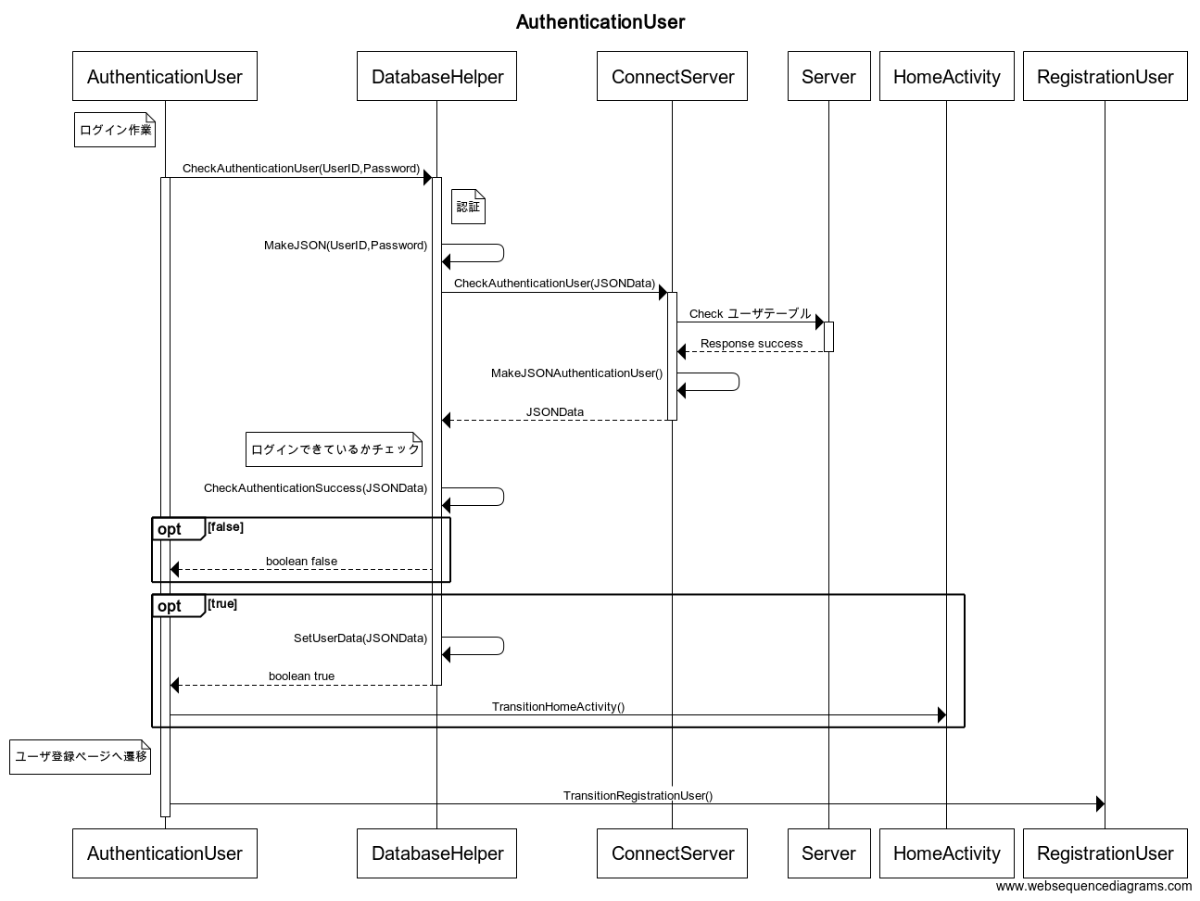
\includegraphics{AuthenticationUser.png}}
  \caption{ログイン認証のシーケンス図}
  \label{tab:AuthenticationUser}
  \end{center}
  \end{figure}
  \subsubsection{ローカルデータベース生成}
  \label{tabs:HomeActivityAndCreateLocalDatabaseSequence}
  アプリのローカルデータベースを生成する際の相互関係を図\ref{tab:HomeActivityAndCreateLocalDatabaseSequence}に示す.
  \begin{figure}[H]
  \begin{center}
  \resizebox{16cm}{!}{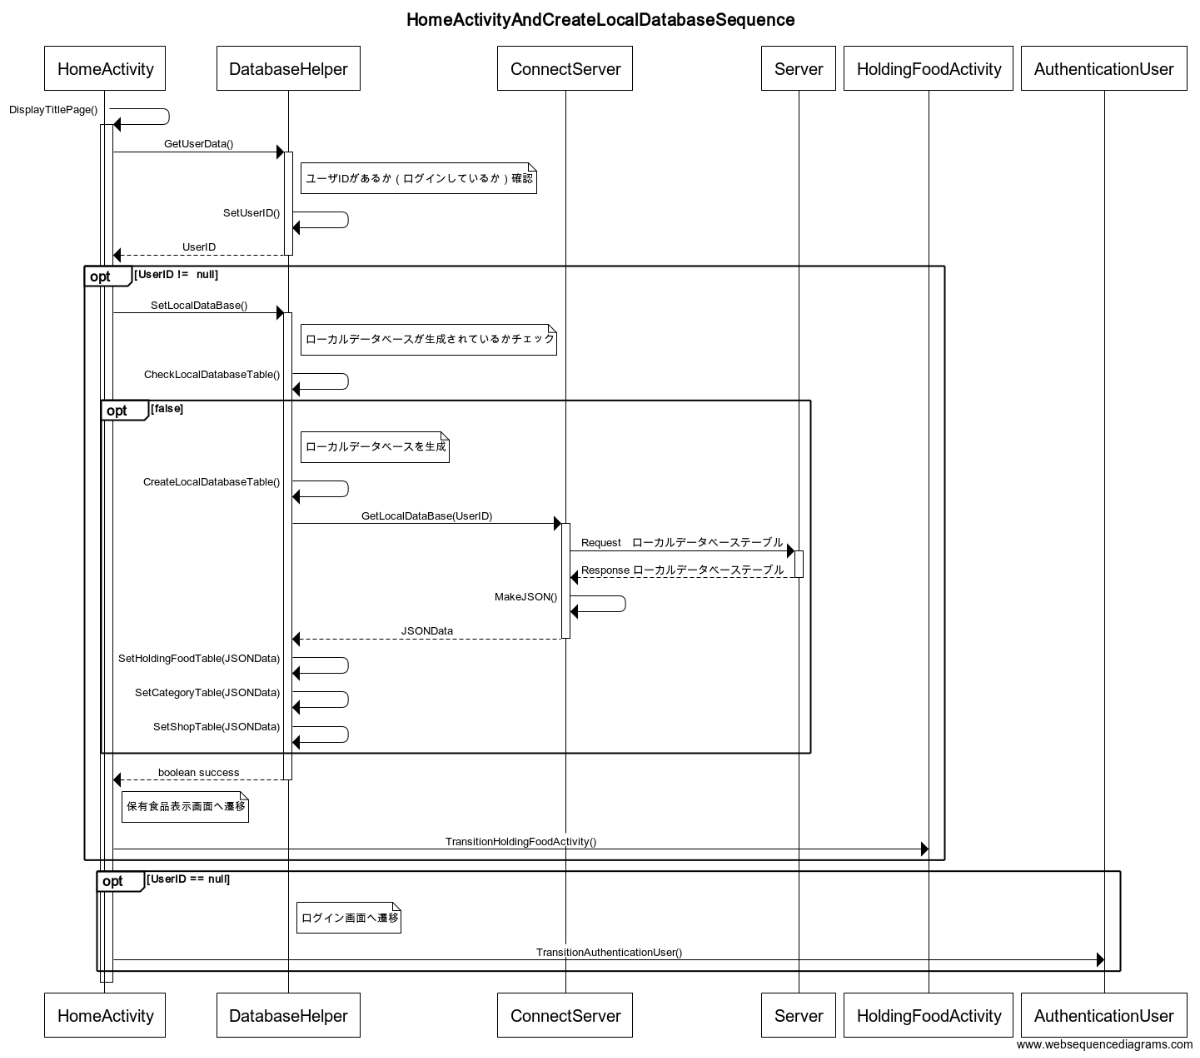
\includegraphics{HomeActivityAndCreateLocalDatabaseSequence.png}}
  \caption{ローカルデータベース生成のシーケンス図}
  \label{tab:HomeActivityAndCreateLocalDatabaseSequence}
  \end{center}
  \end{figure}

  \subsubsection{ユーザ登録画面}
  \label{tabs:RegistrationUserForApplicationSequence}
  ユーザ登録を行う際の相互関係を図\ref{tab:RegistrationUserForApplicationSequence}に示す.
  \begin{figure}[H]
  \begin{center}
  \resizebox{16cm}{!}{\includegraphics{RegistrationUserForApplicationSequence.png}}
  \caption{ユーザ登録のシーケンス図}
  \label{tab:RegistrationUserForApplicationSequence}
  \end{center}
  \end{figure}

  \subsubsection{購入履歴表示画面}
  \label{tabs:PurchaseHistorySequence}
  アプリ上で購入履歴の表示を行う際の相互関係を図\ref{tab:PurchaseHistorySequence}に示す.
  \begin{figure}[H]
  \begin{center}
  \resizebox{16cm}{!}{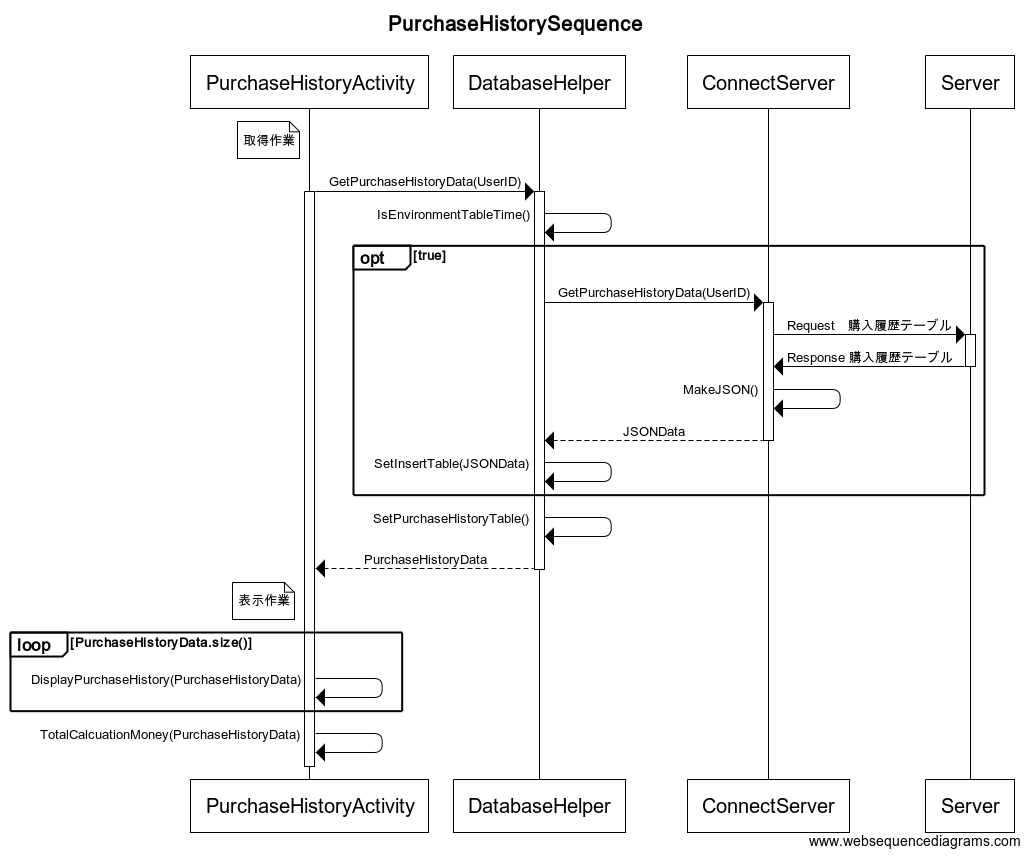
\includegraphics{PurchaseHistorySequence.png}}
  \caption{購入履歴表示のシーケンス図}
  \label{tab:PurchaseHistorySequence}
  \end{center}
  \end{figure}

  \subsubsection{保有食品画面}
  \label{tabs:HoldingFoodSequence}
  アプリ上で保有食品の表示を行う際の相互関係を図\ref{tab:HoldingFoodSequence}に示す.
  \begin{figure}[H]
  \begin{center}
  \resizebox{16cm}{!}{\includegraphics{HoldingFoodSequence.png}}
  \caption{保有食品表示のシーケンス図}
  \label{tab:HoldingFoodSequence}
  \end{center}
  \end{figure}

  \subsubsection{特売情報表示画面}
  \label{tabs:SpecialSaleSequence}
  アプリ上で特売情報の表示を行う際の相互関係を図\ref{tab:SpecialSaleSequence}に示す.
  \begin{figure}[H]
  \begin{center}
  \resizebox{16cm}{!}{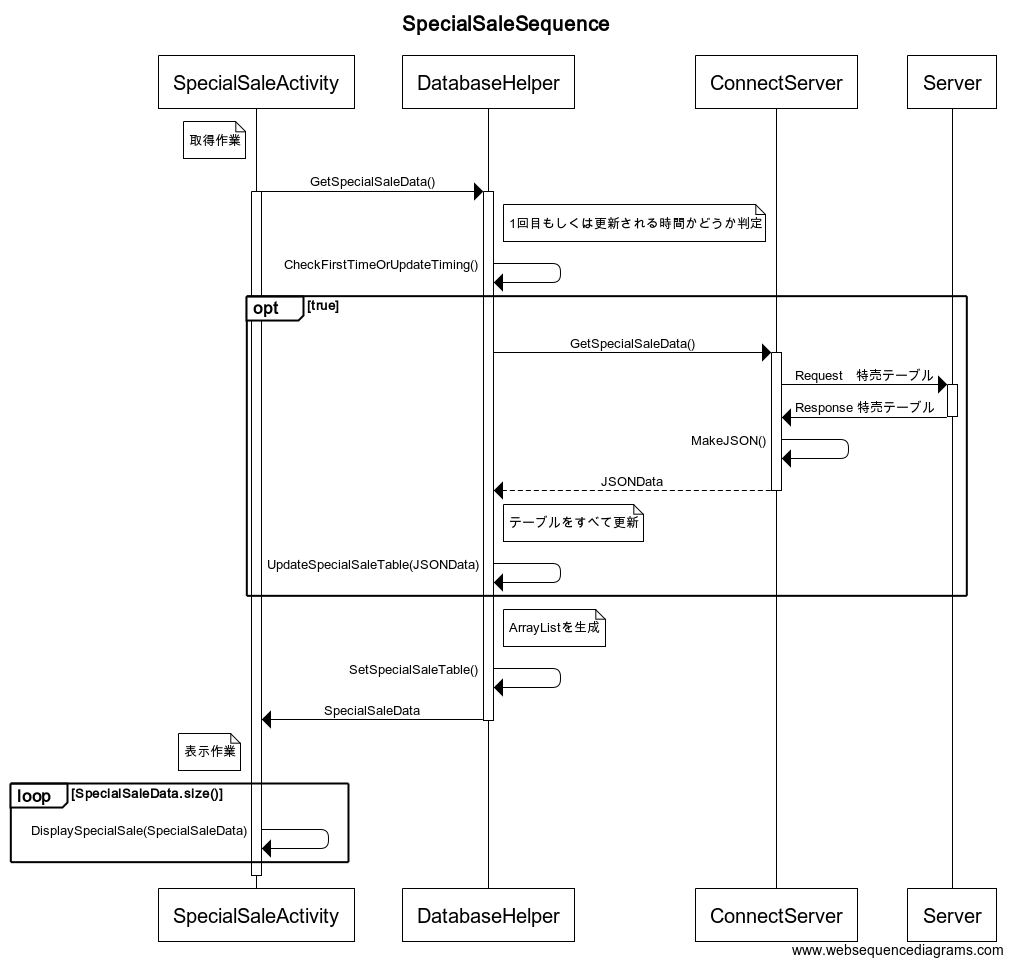
\includegraphics{SpecialSaleSequence.png}}
  \caption{特売情報表示のシーケンス図}
  \label{tab:SpecialSaleSequence}
  \end{center}
  \end{figure}

  \subsubsection{特価情報表示画面}
  \label{tabs:SpecialPriceSequence}
  アプリ上で特価情報の表示を行う際の相互関係を図\ref{tab:SpecialPriceSequence}に示す.
  \begin{figure}[H]
  \begin{center}
  \resizebox{16cm}{!}{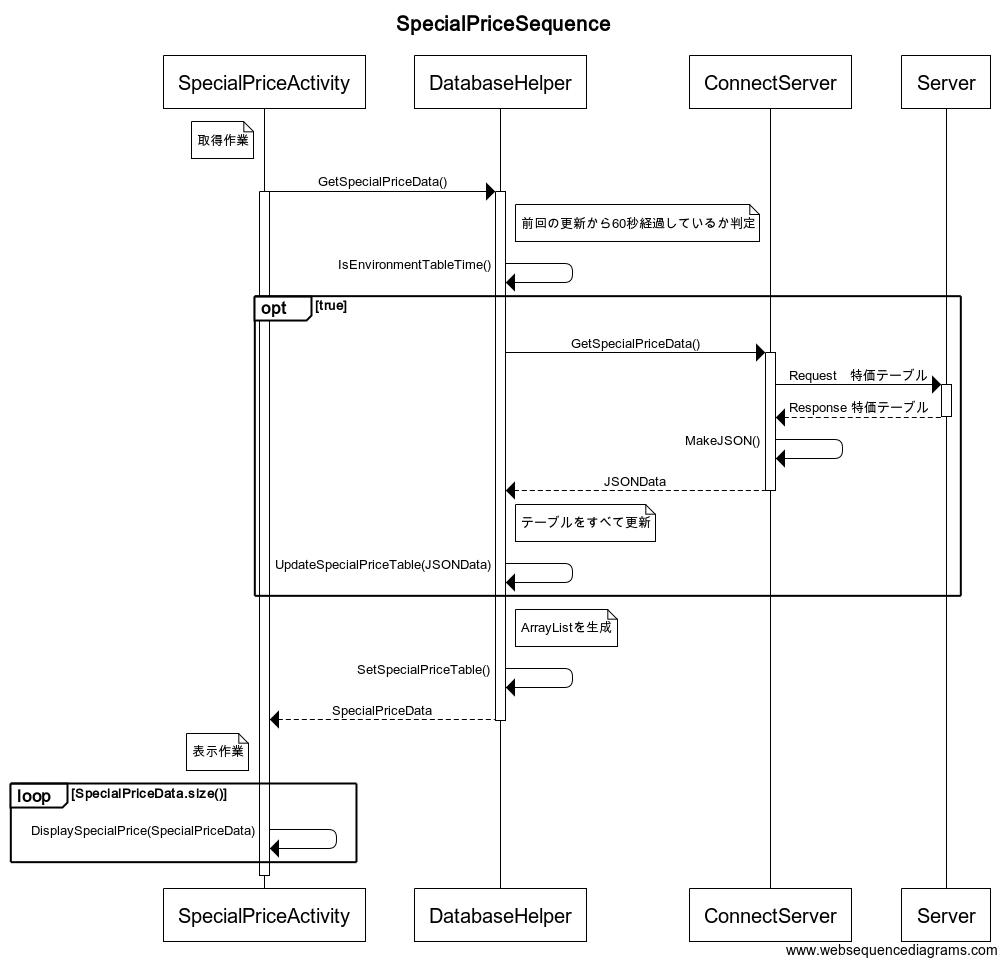
\includegraphics{SpecialPriceSequence.png}}
  \caption{特価情報表示のシーケンス図}
  \label{tab:SpecialPriceSequence}
  \end{center}
  \end{figure}

  \subsubsection{その他画面表示画面}
  \label{tabs:OtherSequence}
  アプリ上でその他画面の表示を行う際の相互関係を図\ref{tab:OtherSequence}に示す.
  \begin{figure}[H]
  \begin{center}
  \resizebox{16cm}{!}{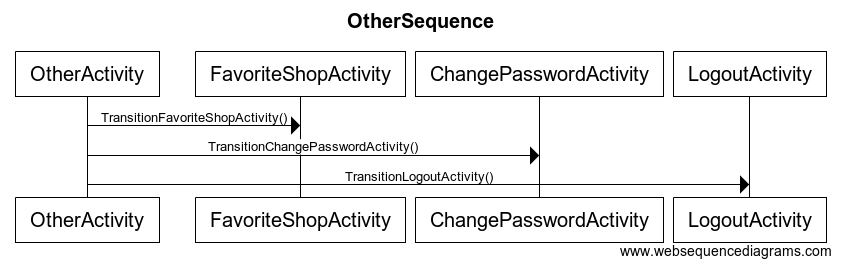
\includegraphics{OtherSequence.png}}
  \caption{その他画面表示のシーケンス図}
  \label{tab:OtherSequence}
  \end{center}
  \end{figure}

  \subsubsection{お気に入り店舗登録画面}
  \label{tabs:FavoriteShopSequence}
  アプリ上でお気に入り店舗の登録を行う際の相互関係を図\ref{tab:FavoriteShopSequence}に示す.
  \begin{figure}[H]
  \begin{center}
  \resizebox{16cm}{!}{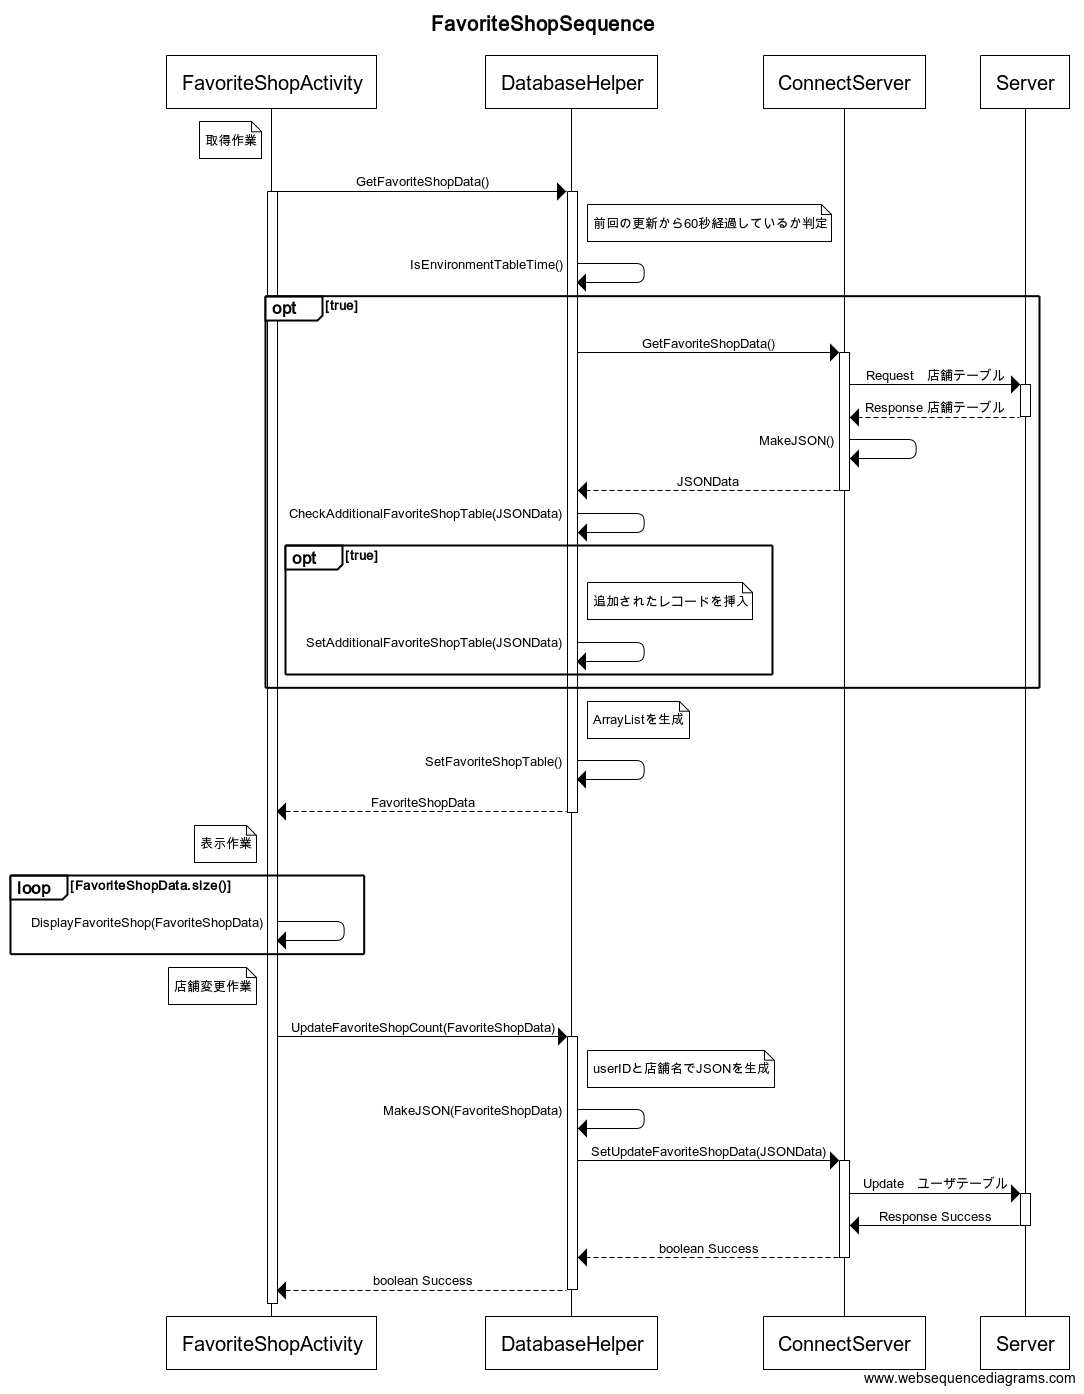
\includegraphics{FavoriteShopSequence.png}}
  \caption{お気に入り店舗登録のシーケンス図}
  \label{tab:FavoriteShopSequence}
  \end{center}
  \end{figure}


  \subsubsection{パスワード変更画面}
  \label{tabs:ChangePasswordSequence}
  アプリ上でパスワードの変更を行う際の相互関係を図\ref{tab:ChangePasswordSequence}に示す.
  \begin{figure}[H]
  \begin{center}
  \resizebox{16cm}{!}{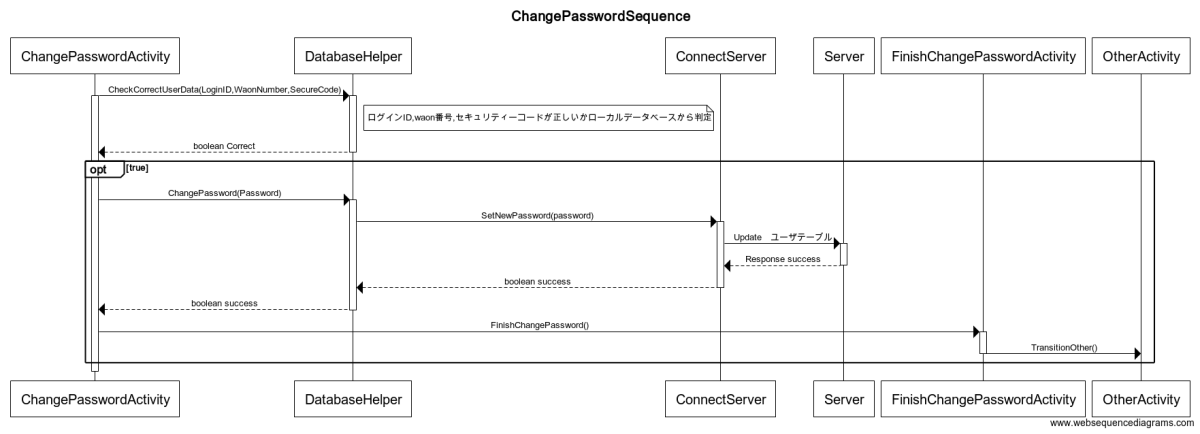
\includegraphics{ChangePasswordSequence.png}}
  \caption{パスワード変更のシーケンス図}
  \label{tab:ChangePasswordSequence}
  \end{center}
  \end{figure}


  \subsubsection{ログアウト画面}
  \label{tabs:LogoutSequence}
  アプリでログアウトを行う際の相互関係を図\ref{tab:LogoutSequence}に示す.
  \begin{figure}[H]
  \begin{center}
  \resizebox{16cm}{!}{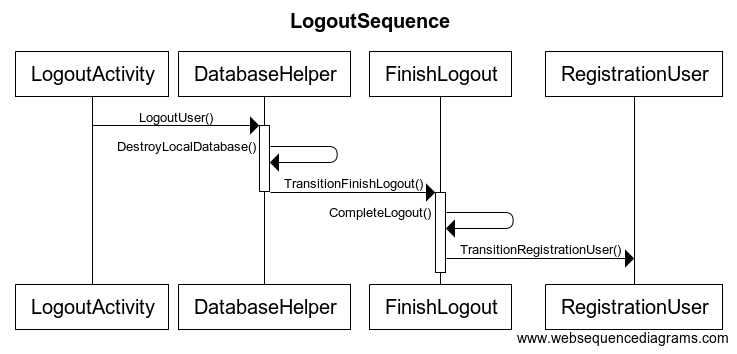
\includegraphics{LogoutSequence.png}}
  \caption{ログアウト画面のシーケンス図}
  \label{tab:LogoutSequence}
  \end{center}
  \end{figure}



  \subsection{シーケンス図(Webページ)}
  	本節では、Webの管理ページを構成するオブジェクト間やサーバとの相互関係を示す。

  	\subsubsection{ログイン画面ユーザ認証}
  	Webのログイン画面でログインを行う際の相互関係を図 \ref{tab:oonishi1}に示す。
  	\begin{figure}[H]
  	\begin{center}
  	\resizebox{16cm}{!}{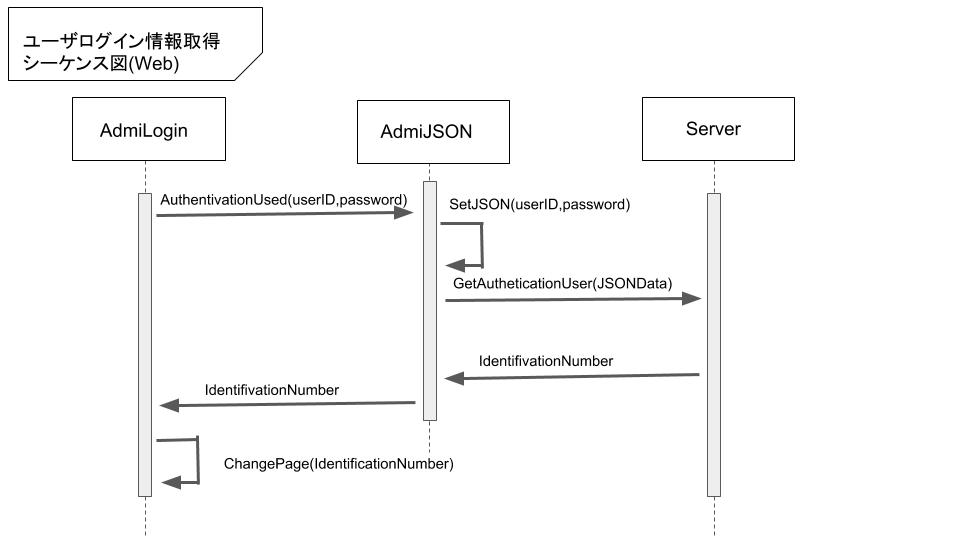
\includegraphics{oonishi1.jpg}}
  	\caption{ログイン画面ユーザ認証のシーケンス図}
  	\label{tab:oonishi1}
  	\end{center}
  	\end{figure}  
  	\subsubsection{店舗情報管理画面店舗登録}
  	Webの店舗情報管理画面で店舗登録を行う際の相互関係を図 \ref{tab:oonishi2}に示す。
  	\begin{figure}[H]
  	\begin{center}
  	\resizebox{16cm}{!}{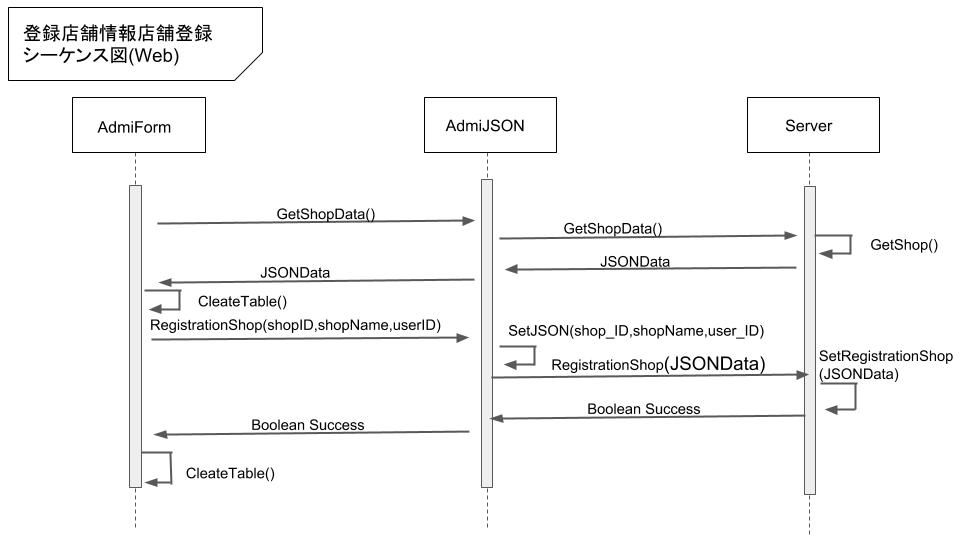
\includegraphics{oonishi2.jpg}}
  	\caption{店舗情報管理画面店舗登録のシーケンス図}
  	\label {tab:oonishi2}
  	\end{center}
  	\end{figure}
  	\subsubsection{店舗情報管理画面店舗更新}
  	Webの店舗情報管理画面で店長の更新を行う際の相互関係を図 \ref{tab:oonishi3}に示す。
  	\begin{figure}[H]
  	\begin{center}
  	\resizebox{16cm}{!}{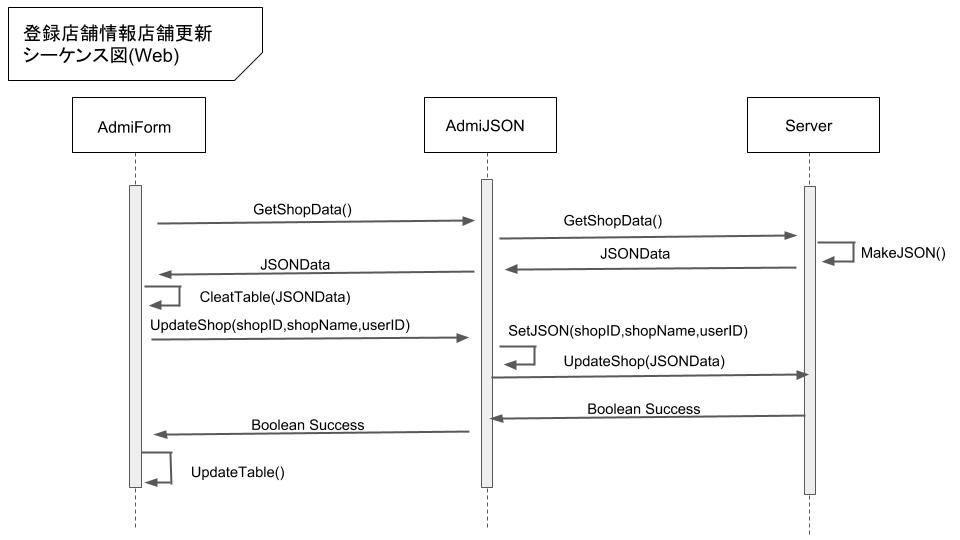
\includegraphics{oonishi3.jpg}}
  	\caption{店舗情報管理画面店舗更新のシーケンス図}
  	\label{tab:oonishi3}
  	\end{center}
  	\end{figure}
  	\subsubsection{店舗情報管理画面店舗削除}
  	Webの店舗情報管理画面で店舗削除を行う際の相互関係を図 \ref{tab:oonishi4}に示す。
  	\begin{figure}[H]
  	\begin{center}
  	\resizebox{16cm}{!}{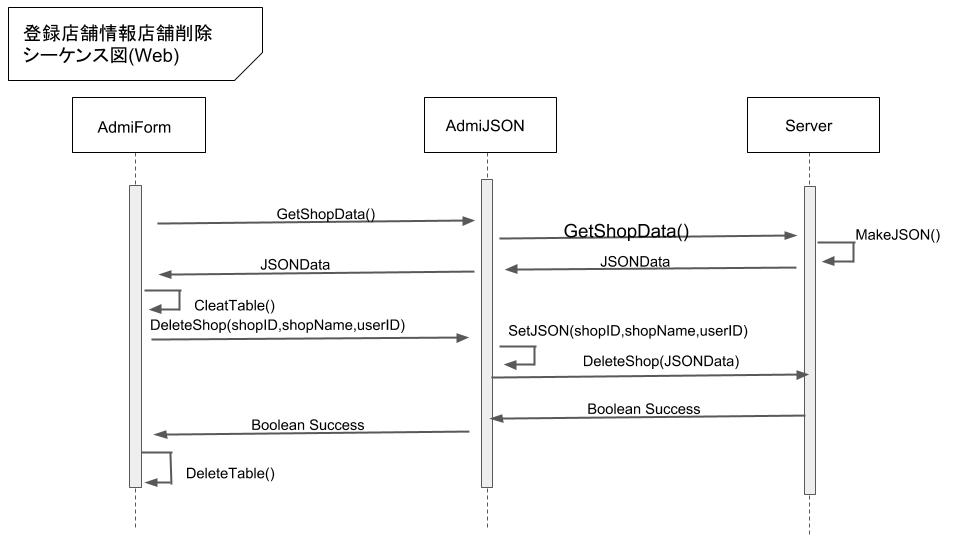
\includegraphics{oonishi4.jpg}}
  	\caption{店舗情報管理画面店舗削除のシーケンス図}
  	\label{tab:oonishi4}
  	\end{center}
  	\end{figure}

  	\subsubsection{特売情報管理画面特売情報登録}
  	Webの特売情報管理画面で特売情報登録を行う際の相互関係を図 \ref{tab:oonishi21}に示す。
  	\begin{figure}[H]
  	\begin{center}
  	\resizebox{16cm}{!}{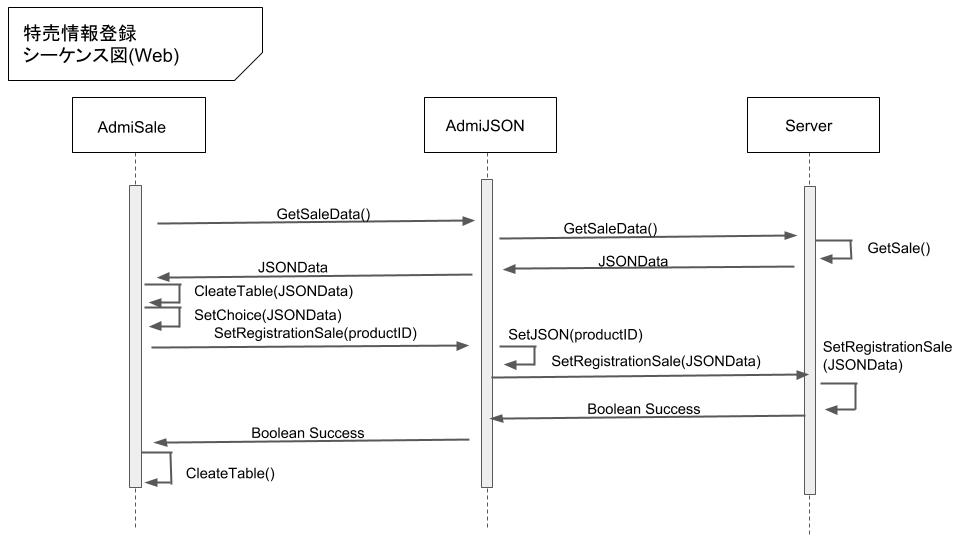
\includegraphics{oonishi21.jpg}}
  	\caption{特売情報管理画面特売情報登録のシーケンス図}
  	\label{tab:oonishi21}
  	\end{center}
  	\end{figure}
  	\subsubsection{特売情報管理画面特売情報削除}
  	Webの特売情報管理画面で特売情報削除を行う際の相互関係を図 \ref{tab:oonishi22}に示す。
  	\begin{figure}[H]
  	\begin{center}
  	\resizebox{16cm}{!}{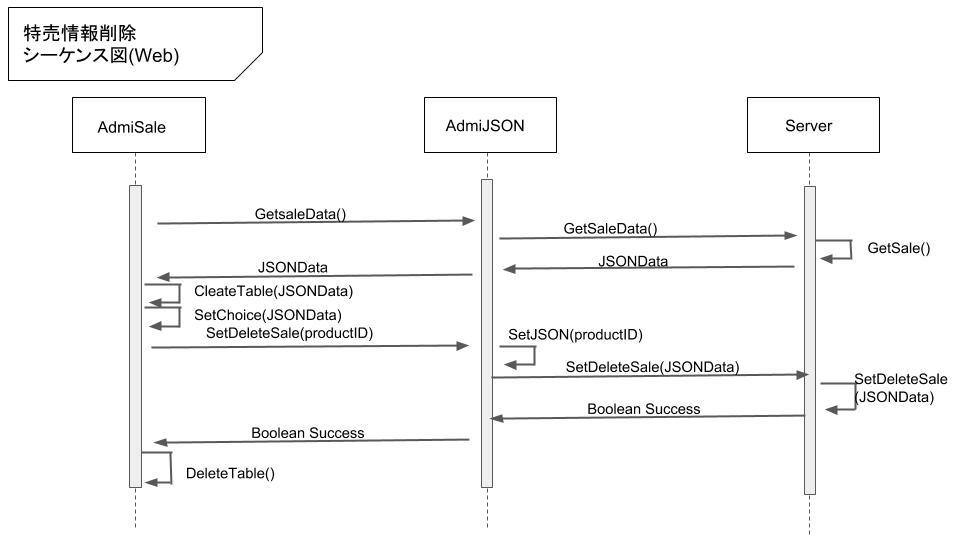
\includegraphics{oonishi22.jpg}}
  	\caption{特売情報管理画面特売情報削除のシーケンス図}
  	\label{tab:oonishi22}
  	\end{center}
  	\end{figure}
  	\subsubsection{特価情報管理画面特価情報登録}
  	Webの特価情報管理画面で特価情報登録を行う際の相互関係を図 \ref{tab:oonishi23}に示す。
  	\begin{figure}[H]
  	\begin{center}
  	\resizebox{16cm}{!}{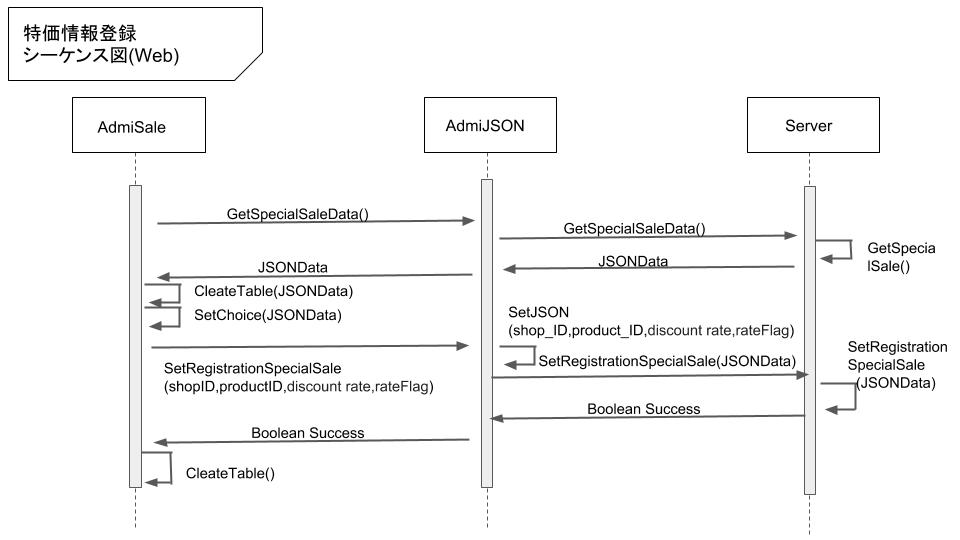
\includegraphics{oonishi23.jpg}}
  	\caption{特売情報管理画面特売情報登録のシーケンス図}
  	\label{tab:oonishi23}
  	\end{center}
  	\end{figure}
  	\subsubsection{特価情報管理画面特価情報更新}
  	Webの特価情報管理画面で特価情報更新を行う際の相互関係を図 \ref{tab:oonishi24}に示す。
  	\begin{figure}[H]
  	\begin{center}
  	\resizebox{16cm}{!}{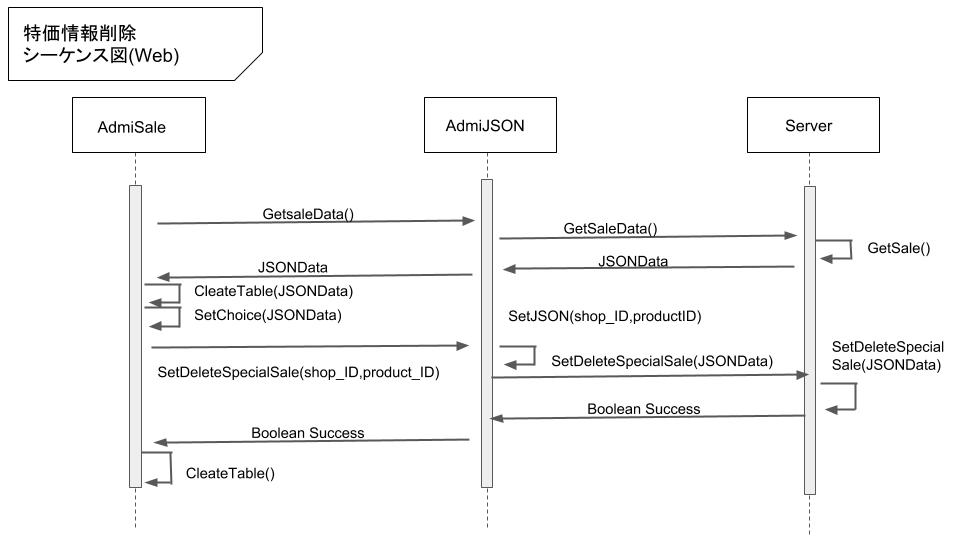
\includegraphics{oonishi24.jpg}}
  	\caption{特売情報管理画面特売情報更新のシーケンス図}
  	\label{tab:oonishi24}
  	\end{center}
  	\end{figure}
  	\subsubsection{特価情報管理画面特価情報削除}
  	Webの特価情報管理画面で特価情報削除を行う際の相互関係を図 \ref{tab:oonishi25}に示す。
  	\begin{figure}[H]
  	\begin{center}
  	\resizebox{16cm}{!}{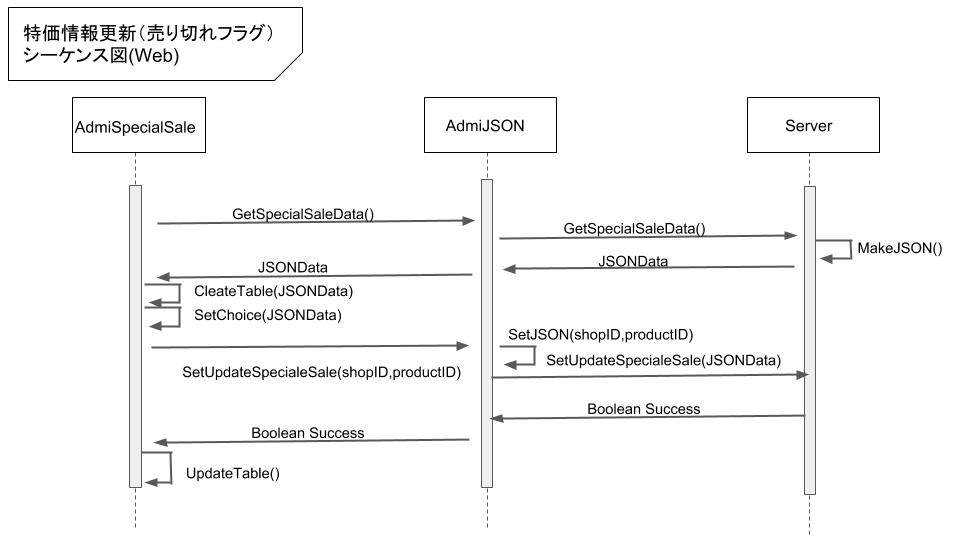
\includegraphics{oonishi25.jpg}}
  	\caption{特売情報管理画面特売情報削除のシーケンス図}
  	\label{tab:oonishi25}
  	\end{center}
  	\end{figure}



\section{データベース設計}
本節では,本システムで用いるデータベースにおける各テーブルの設計と本システムで用いる各画面の処理用SQL文について記述する.各テーブルの関係性を示すER図を以下の図\ref{tab:ER}に示す.
\begin{figure}[H]
\begin{center}
\resizebox{16cm}{!}{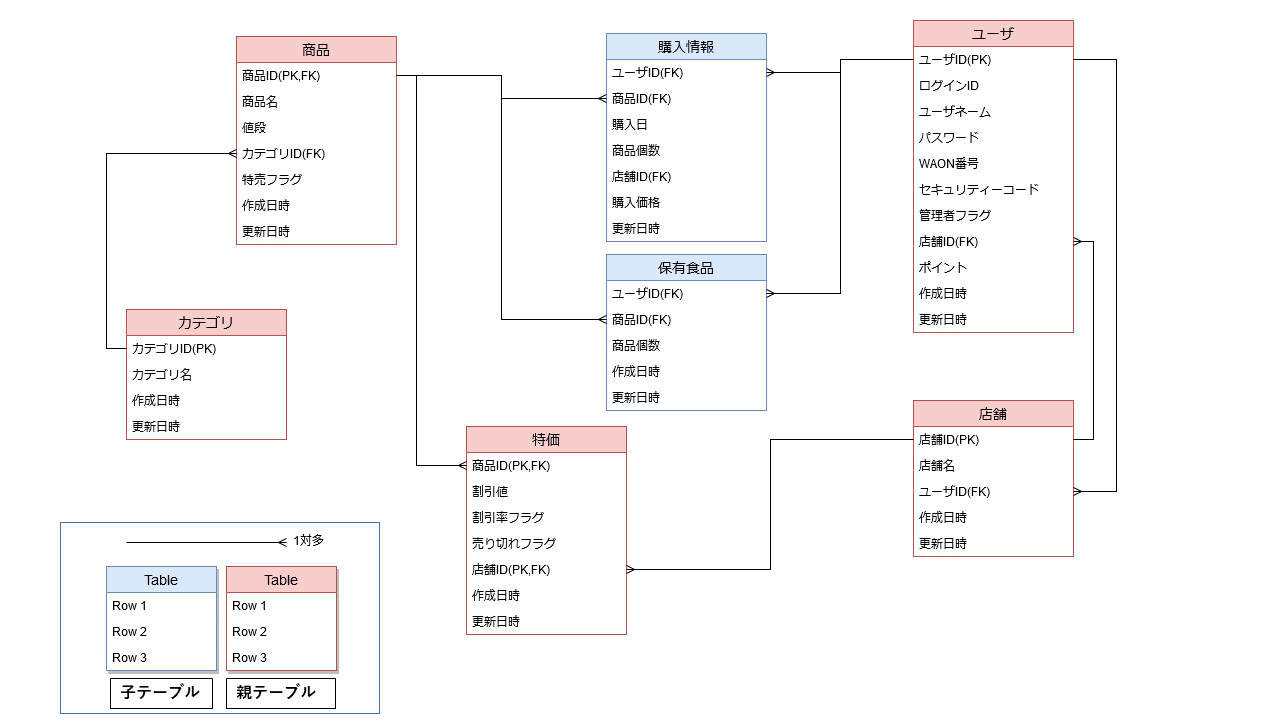
\includegraphics{DB_R.PNG}}
\caption{本システムで用いるデータベースのER図}
\label{tab:ER}
\end{center}
\end{figure}

\subsection{テーブル設計}
本小節では,本システムで用いるデータベースにおける各テーブルの設計について画像および各レコードの説明を付与して解説する.
\subsubsection{購入テーブル}
購入テーブルではユーザの購入に関する情報を管理する。このテーブルの詳細については表\ref{table_buy}に示す。


\begin{figure}[H]
  \begin{center}
    \includegraphics[width=15cm]{table_buy.png} \\
    \caption{購入テーブル}
    \label{table_buy}
  \end{center}
\end{figure}
購入テーブルを作成するためのCREATE文を下記に示す。

\begin{screen}
CREATE TABLE buy (\\
  user\_id CHAR(7) NOT NULL,\\
  product\_id CHAR(10) NOT NULL,\\
  num INTEGER,\\
  store\_id CHAR(3) NOT NULL,\\
  price INTEGER,\\
  createDate DATE,\\
  updateDate DATE,\\
  PRIMARY KEY (user\_id, product\_id, createDate),\\
  FOREIGN KEY (store\_id) REFERENCES stores\\
);
\end{screen}
\begin{itemize}
\item ユーザID

  自テーブルの複合主キーである。ユーザテーブルを参照する際の外部キーである。ユーザを識別するための値である。(例:0000001)

\item 商品ID

  自テーブルの複合主キーである。商品テーブルを参照する際の外部キーである。商品を識別する値である。(例:1234567890)

\item 商品個数

  購入した商品の個数を示す値である。(例:10)

\item 店舗ID

  店舗テーブルを参照する際の外部キーである。店舗を識別するための値である。(例:001)

\item 購入価格

  購入した商品の値段を示す値である。(例:12345)

\item 作成日時

  自テーブルの複合主キーである。レコードを作成した日付・時刻を示す値である。(例:2018-12-25 12:59:18)

\item 更新日時

  レコードを更新した日付・時刻を示す値である。(例:2018-12-25 12:59:18)

\end{itemize}


\subsubsection{ユーザテーブル}
ユーザテーブルでは,登録したユーザについて関する情報を管理する。このテーブルの詳細について表\ref{table_users}に示す。
\begin{figure}[H]
  \begin{center}
    \includegraphics[width=15cm]{table_users.png} \\
    \caption{ユーザテーブル}
    \label{table_users}
  \end{center}
\end{figure}
ユーザテーブルを作成するためのCREATE文を下記に示す。
\begin{screen}
CREATE TABLE users (\\
  user\_id CHAR(7) NOT NULL,\\
  loginid CHAR VARYING(10),\\
  name NCHAR VARYING(15),\\
  ruby NCHAR VARYING(30),\\
  Password CHAR(16),\\
  waon CHAR(16),\\
  security CHAR(16),\\
  admFlg CHAR(1),\\
  store\_id CHAR(3),\\
  points INTEGER,\\
  createDate DATE,\\
  updateDate DATE,\\
  PRIMARY KEY (user\_id),\\
  FOREIGN KEY (store\_id) REFERENCES stores\\
);
\end{screen}
\begin{itemize}

\item ユーザID

  ユーザID自テーブルの主キーである。ユーザテーブルを参照する際の外部キーである。ユーザを識別する値である。(例:0000001)

\item ログインID

  ユーザのログインIDを示す値である。(例:yamada)

\item ユーザネーム

  ユーザのログインIDを示す値である。値は15文字以下の全角文字にて構成される。(例:山田)

\item フリガナ

  ユーザネームのフリガナを示す値である。値は30文字以下の全角文字にて構成される。(例:ヤマダ)

\item パスワード

  ユーザがログイン時に使用するパスワードを示す値である。(例:Shjkas1029384756)

\item WAON番号

  ユーザの所有するWAONカードのWAON番号を示す値である。(例:1234567890123456)

\item セキュリティコード

  ユーザの所有するWAONカードのセキュリティコードを示す値である。(例:1234567890123456)

\item 管理者フラグ

  ユーザが管理者か店長かどうか識別する値である。(0:管理者、1:店長)

\item 店舗ID

  店舗テーブルを参照する際の外部キーである。店舗を識別するための値である。(例:001)

\item ポイント

  ユーザの所有するWAONポイントを示す値である。 (例:120)

\item 作成日時

  レコードを作成した日付・時刻を示す値である。(例:2018-12-25 12:59:18)

\item 更新日時

  レコードを更新した日付・時刻を示す値である。(例:2018-12-25 12:59:18)
\end{itemize}


\subsubsection{商品テーブル(products)}

商品テーブルでは商品に関する情報を管理する。このテーブルの詳細については表\ref{table_products}に示す。

\begin{figure}[H]
  \begin{center}
    \includegraphics[width=15cm]{table_products.png} \\
    \caption{商品テーブル}
    \label{table_products}
  \end{center}
\end{figure}

商品テーブルを作成するためのCREATE文を下記に示す。
\begin{screen}
CREATE TABLE products (\\
  product\_id CHAR(10),\\
  name NCHAR VARYING(50),\\
  price INTEGER(5),\\
  category\_id CHAR(2),\\
  bargainFlg CHAR(1),\\
  createDate,\\
  updateDate,\\
  PRIMARY KEY(product\_id),\\
  FOREIGN KEY(category\_id) REFERENCES category,\\
);
\end{screen}
\begin{itemize}
\item 商品ID\par
  自テーブルの主キーである。商品を識別するための値である。(例:1234567890)

\item 商品名\par
  商品の名前を示す値である。(例:牛乳)

\item 値段\par
  商品の値段を示す値である。(例:00108)

\item カテゴリID\par
  カテゴリテーブルを参照する際の外部キーである。商品のカテゴリを示す値である。(例:10)

\item 特売フラグ\par
  その商品が特売商品であるかを示す値である。(例:1)

\item 作成日時\par
  レコードを作成した日付・時刻を示す値である。(例:2018-12-25 12:59:18)

\item 更新日時\par
  レコードを更新した日付・時刻を示す値である。(例:2018-12-25 12:59:18)
\end{itemize}


\subsubsection{保有食品テーブル(hold)}

保有食品テーブルではアプリ利用者が保有している食品に関する情報を管理する。このテーブルの詳細については表\ref{table_hold}に示す。

\begin{figure}[H]
  \begin{center}
    \includegraphics[width=15cm]{table_hold.png} \\
    \caption{保有食品テーブル}
    \label{table_hold}
  \end{center}
\end{figure}

保有食品テーブルを作成するためのCREATE文を下記に示す。
\begin{screen}
  CREATE TABLE hold (\\
    user\_id CHAR(7),\\
    product\_id CHAR(10),\\
    num INTEGER,\\
    createDate,\\
    updateDate,\\
    FOREIGN KEY(user\_id) REFERENCES users,\\
    FOREIGN KEY(product\_id) REFERENCES products\\
  );
\end{screen}
\begin{itemize}
\item ユーザID\par
  ユーザテーブルを参照する際の外部キーである。ユーザを識別する値である。(例:0000001)

\item 商品ID\par
  商品テーブルを参照する際の外部キーである。商品を識別するための値である。(例:1234567890)

\item 商品個数\par
  購入した商品の個数を示す値である。(例:10)

\item 作成日時\par
  レコードを作成した日付・時刻を示す値である。(例:2018-12-25 12:59:18)

\item 更新日時\par
  レコードを更新した日付・時刻を示す値である。(例:2018-12-25 12:59:18)
\end{itemize}
\subsubsection{店舗テーブル(store)}
店舗テーブルではマルナカの店舗に関する情報を管理する。このテーブルの詳細については表に示す。
% ここにテーブルの表をはる
\begin{figure}[H]
  \begin{center}
    \includegraphics[width=15cm]{table_stores.png} \\
    \caption{店舗テーブル}
    \label{table_store}
  \end{center}
\end{figure}
店舗テーブルを作成するためのCREATE文を下記に示す。
% ここにCREATE文を示す
\begin{screen}
  CREATE TABLE stores ( \\
    store\_id CHAR(3), \\
    name NCHAR VARYING(18), \\
    user\_id CHAR(7), \\
    createDate DATE, \\
    updateDate DATE, \\
    PRIMARY KEY (store\_id), \\
    FOREIGN KEY (user\_id) REFERENCES users \\
  );
\end{screen}
\begin{itemize}
\item 店舗ID \par
  \indent 店舗テーブルの主キーである。値は、3文字の固定長半角英数字で構成されている。(例:015)
\item 店舗名 \par
  \indent マルナカの店舗名を示す値である。値は、18文字の可変長全角文字で構成されている。(例:マルナカ南国店)
\item ユーザID \par
  \indent ユーザテーブルを参照する際の外部キーである。値は、7文字の固定長半角英数字で構成されている。(例:0000026)
\item 作成日時 \par
  \indent レコードを作成した日付・時刻を示す値である。(例:2018-12-25 12:59:18)
  \item 更新日時 \par
    \indent レコードを更新した日付・時刻を示す値である。(例:2018-12-25 12:59:18)
\end{itemize}


\subsubsection{カテゴリテーブル(category)}
カテゴリテーブルでは商品のカテゴリに関する情報を管理する。このテーブルの詳細については表\ref{table_category}に示す。カテゴリテーブルを作成するためのCREATE文を下記に示す。

\begin{figure}[H]
  \begin{center}
    \includegraphics[width=15cm]{table_category.png} \\
    \caption{カテゴリテーブル}
    \label{table_category}
  \end{center}
\end{figure}

\begin{screen}
  CREATE TABLE category( \\
    category\_id CHAR(2) NOT NULL, \\
    name NCHAR(10), \\
    product\_id\ CHAR(10), \\
    createDate DATE, \\
    updateDate DATE, \\
    PRIMARY KEY (category\_id), \\
    FOREIGN KEY (product\_id) REFERENCES products \\
  );
\end{screen}

\begin{itemize}
\item カテゴリID\par
  カテゴリテーブルを参照する際の外部キーである。商品のカテゴリを示す値である。(例:10)
\item カテゴリ名\par
  商品のカテゴリの名前を示す値である。(例:飲料水)
\item 商品ID\par
  商品テーブルを参照する際の外部キーである。商品を識別するための値である。(例:1234567890)
\item 作成日時\par
  レコードを作成した日付・時刻を示す値である。(例:2018-12-25 12:59:18)
\item 更新日時\par
  レコードを更新した日付・時刻を示す値である。(例:2018-12-25 12:59:18)
\end{itemize}
\subsubsection{特価テーブル(sp\_price)}
特価テーブルでは特価に関する情報を管理する。このテーブルの詳細については表\ref{table_sp_price}に示す。特価テーブルを作成するためのCREATE文を下記に示す。
\begin{figure}[H]
  \begin{center}
    \includegraphics[width=15cm]{table_sp_price.png} \\
    \caption{特価テーブル}
    \label{table_sp_price}
  \end{center}
\end{figure}

\begin{screen}
  CREATE TABLE sp\_price( \\
    product\_id CHAR(10) NOT NULL, \\
    discntVal INTEGER(3), \\
    rateFlg CHAR(1), \\
    soldOutFlg CHAR(1), \\
    store\_id CHAR(3) NOT NULL, \\
    createDate DATE, \\
    updateDate DATE, \\
    PRIMARY KEY (product\_id,store\_id), \\
    FOREIGN KEY (product\_id) REFERENCES product, \\
    FOREIGN KEY (store\_id) REFERENCES store \\
  );
\end{screen}

\begin{itemize}
\item 商品ID\par
  商品テーブルを参照する際の外部キーである。商品を識別するための値である。(例:1234567890)
\item 割引値\par
  商品が割引されるとき、いくら割引されるかを示す値である。(例:-30)
\item 割引率フラグ\par
  商品を割引するとき円引きか\%引きかを識別するためのフラグである。(例:0)
\item 売り切れフラグ\par
  割引された商品が売り切れているか売れ残っているか識別するための値である。(例:0)
\item 店舗ID\par
  店舗テーブルを参照する際の外部キーである。店舗を識別するための値である。(例:005)
\item 作成日時\par
  レコードを作成した日付・時刻を示す値である。(例:2018-12-25 12:59:18)
\item 更新日時\par
  レコードを更新した日付・時刻を示す値である。(例:2018-12-25 12:59:18)
\end{itemize}


\subsection{各画面処理}

本章節では、各画面ごとに行われる処理について示す。


\subsubsection{新規登録画面}
新規登録画面でユーザテーブルにデータを挿入するSQL文を下記に示す。
\begin{screen}
  //値の取得// \\
  SELECT MAX(CAST(user\_id) AS INTEGER) \\
   FROM users; \\

  //入力値// \\
  \$1 = ユーザIDの最大値+1した値 \\
  \$2 = ログインID(入力フォーラムによる値) \\
  \$3 = ユーザネーム(入力フォーラムによる値) \\
  \$4 = フリガナ(入力フォーラムによる値) \\
  \$5 = パスワード(入力フォーラムによる値) \\
  \$6 = WAON番号(入力フォーラムによる値) \\
  \$7 = セキュリティコード(入力フォーラムによる値) \\
  \$8 = ポイント \\
  \$9 = システム日付 \\

  //値の挿入//\\
  INSERT INTO users VALUES ( \\
    \$1, \$2, \$3, \$4, \$5, \$6, \$7, \\
    '0', NULL, \$8, \$9, \$9 \\
  );
\end{screen}


\subsubsection{ログイン画面(アプリ)}
ログイン画面でログインするための情報を取得するSQL文を以下に示す。

\begin{screen}
  ///入力値///\\
  \$1 = ユーザID\\
  \$2 = パスワード\\
  \\
  ///値の取得///\\
   SELECT user\_id, name, points, store\_id\\
    FROM users\\
    WHERE user\_id = \$1\\
    AND Password = \$2
\end{screen}


\subsubsection{購入履歴画面}
購入履歴画面で購入した商品のデータを取得するSQL文を下記に示す。
\begin{screen}
  //入力値// \\
  \$1 = アプリからのユーザID \\

  //値の取得// \\
  SELECT b.name, a.num, a.price, a.createDate \\
   FROM buy a, products b \\
   WHERE a.product\_id = b.product\_id \\
    AND a.user\_id = \$1;
\end{screen}


\subsubsection{保有食品画面}
保有食品画面で必要な情報を取得するSQL文を下記に示す。
\begin{screen}
   ///入力値///\\
  \$1 = アプリから受け取ったユーザID
  \\
   ///SQL///\\
  SELECT b.name, a.num, a.createDate\\
    FROM hold a, products b\\
    WHERE a.product\_id = b.product\_id\\
    AND a.user\_id = \$1
\end{screen}

保有食品画面で食品を削除するSQL文を下記に示す。
\begin{screen}
   ///入力値///\\
  \$1 = アプリから受け取ったユーザID\\
  \$2 = アプリから受け取った食品ID\\
  \$3 = アプリから受け取った購入日\\
  \\
   ///SQL///\\
  DELETE *\\
    FROM hold a\\
    WHERE a.user\_id = \$1\\
    AND a.product\_id = \$2\\
    AND a.create = \$3
\end{screen}

保有食品画面で食品を更新するSQL文を下記に示す。
\begin{screen}
   ///入力値///\\
  \$1 = アプリから受け取った商品個数\\
  \$2 = システム日付\\
  \$3 = アプリから受け取ったユーザID\\
  \\
   ///SQL///\\
  UPDATE hold\\
    SET num = \$1\\
    updateDate = \$2\\
    WHERE user\_id = \$3
\end{screen}


\subsubsection{特売・特価情報閲覧画面}
特売・特価情報閲覧画面で特売・特価情報を取得するSQL文を下記に示す。
\begin{screen}
  SELECT name, price\\
    FROM products\\
    WHERE bargainFlg = `1`
\end{screen}

\begin{screen}
   ///入力値///\\
  \$1 = 店舗ID\\
  \\
  ///値の取得///\\
   SELECT a.name, b.discntVal, b.rateFlg, b.soldOutFlg, c.name\\
    FROM products a, sp\_price b stores c\\
    WHERE a.product\_id = b.product\_id\\
    AND b.store\_id = c.store\_id\\
    AND b.store\_id = \$1
\end{screen}


\subsubsection{ログイン画面(Web)}
ログイン画面でログインするための情報を取得するSQL文を以下に示す。

\begin{screen}
  ///入力値///\\
  \$1 = ユーザID\\
  \$2 = パスワード\\
  \\
  ///値の取得///\\
   SELECT admFlg\\
    FROM users\\
    WHERE user\_id = \$1\\
    AND Password = \$2
\end{screen}


\subsubsection{特売情報管理画面}
特売情報管理画面で特売情報を更新するSQL文を下記に示す。
\begin{screen}
   ///入力値///\\
  \$1 = 特売フラグの変更値(追加 = 1, 削除 = 0)\\
  \$2 = Webページから受けっとった商品ID
  \\
   ///SQL///\\
  UPDATE products\\
    SET bargainFlg = \$1\\
    WHERE productt\_id = \$2
\end{screen}


\subsubsection{特価情報管理画面} 
特価情報管理画面で特価情報を取得するSQL文を以下に示す。

\begin{screen}
  ///値の取得///\\
    SELECT a.product\_id, b.name, b.price, b.discntVal\\
    FROM sp\_price a, products b
\end{screen}

特価情報管理画面でデータを特価テーブルに挿入するSQL文を以下に示す。

\begin{screen}
   ///入力値///\\
   \$1 = 商品ID\\
   \$2 = 割引値\\
   \$3 = 割引率フラグ\\
   \$4 = 店舗フラグ\\
   \$5 = システム日付\\
  \\
  ///値の挿入///\\
   INSERT INTO sp\_price VALUES (\\
    \$1, \$2, \$3, '0', \$4, \$5, \$5\\
  );
\end{screen}

特価情報管理画面で特価情報を更新するSQL文を以下に示す。

\begin{screen}
  ///入力値///\\
  \$1 = 売り切れフラグ\\
  \$2 = 店舗ID\\
  \\
  ///値の更新///\\
   UPDATE sp\_price\\
    SET soldOutFlg = `1`\\
    WHERE product\_id = \$1\\
    AND store\_id = \$2
\end{screen}

特価情報管理画面で特価情報を一部削除するSQL文を以下に示す。

\begin{screen}
  ///入力値///\\
  \$1 = 商品ID\\
  \$2 = 店舗ID\\
  \\
  ///値の削除///\\
   DELETE *\\
    FROM sp\_price\\
    WHERE product\_id = \$1\\
    AND store\_id = \$2
\end{screen}

特価情報管理画面で特価情報を全部削除するSQL文を以下に示す。

\begin{screen}
  ///入力値///\\
  \$1 = 店舗ID\\
  \\
  ///値の削除///\\
   DELETE *\\
    FROM sp\_price\\
    WHERE store\_id = \$1
\end{screen}


\subsubsection{店舗登録画面}
店舗登録画面で店舗の情報を取得するSQL文を下記に示す。
\begin{screen}
  SELECT store\_id, name, use\_id \\
   FROM stores;
\end{screen}
新たに店舗を登録する場合のデータ挿入のSQL文を下記に示す。
\begin{screen}
  //値の取得// \\
  SELECT MAX(CAST(store\_id) AS INTEGER) \\
   FROM stores; \\

  //入力値// \\
  \$1 = 店舗IDの最大値+1した値 \\
  \$2 = 店舗名(入力フォーラムによる値) \\
  \$3 = ユーザID(入力フォーラムによる値) \\
  \$4 = システム日付 \\

  //値の挿入// \\
  INSERT INTO stores VALUES ( \\
    \$1, \$2, \$3, \$4 \\
  );
\end{screen}
登録してある店舗を削除する場合のデータ削除のSQL文を下記に示す。
\begin{screen}
  //入力値// \\
  \$1 = Web側からの店舗ID \\
  \$2 = Web側からのユーザID \\

  //値の削除// \\
  DELETE * \\
   FROM stores \\
   WHERE store\_id = \$1; \\

  DELETE * \\
   FROM users \\
   WHERE user\_id = \$2;
\end{screen}
登録している店舗の情報を変更した場合のデータ更新のSQL文を下記に示す。
\begin{screen}
  //入力値// \\
  \$1 = Web側からの店舗ID \\
  \$2 = Web側からのユーザID \\
  \$3 = システム日付 \\

  //値の更新// \\
  UPDATE stores \\
   SET user\_id = \$2, updateDate = \$3 \\
   WHERE store\_id = \$1;
\end{screen}


\subsection{自動更新処理}

\subsubsection{パスワード更新処理}
パスワード更新時のSQLを以下に示す。
\begin{screen}
  /////入力フォーラムによる値/////\\
  \$1 = パスワード\\
  \$2 = システム日付\\
  \$3 = ユーザID\\
  \\
  /////値の取得/////\\
  UPDATE user\\
    SET pass = \$1,updateDate = \$3\\
   WHERE user\_id = \$2;
\end{screen}


\subsubsection{店舗更新処理}
店舗更新時のSQLを以下に示す。
\begin{screen}
  /////入力フォーラムによる値/////\\
  \$1 = 店舗ID\\
  \$2 = ユーザID\\
  \$3 = システム日付\\
  \\
  /////値の取得/////\\
  UPDATE user\\
    SET store\_id = \$1,updateDate = \$2\\
    WHERE user\_id = \$3;
\end{screen}


\subsubsection{パスワード変更処理}
パスワード変更時のSQLを以下に示す。
\begin{screen}
  /////入力フォーラムによる値/////\\
  \$1 = アプリからのログインID\\
  \$2 = アプリからのWAON番号\\
  \$3 = アプリからのセキュリティコード\\
  \\
  /////値の取得/////\\
  SELECT user\_id\\
    FROM user\\
    WHERE login\_id = \$1\\
    AND waon = \$2\\
    AND security = \$3;
\end{screen}
\end{document}
